\begin{tikzpicture}[scale=.2, anchor=west]
\node[draw opacity=0, fill opacity=0, anchor=south west] (dummyL) at (-3, -15){};
\node[draw=black, rectangle split, anchor=south west, rectangle split parts=3] (sn0x26141c0) at ([xshift=2cm]dummyL){
\begin{tikzpicture}[scale=.2]
\node[circle, scale=0.75, fill] (tid0) at (4.5,1.5){};
\node[circle, scale=0.75, fill] (tid1) at (2.25,3){};
\node[circle, scale=0.75, fill, red] (tid4) at (0.75,4.5){};
\node[circle, scale=0.75, fill] (tid5) at (2.25,4.5){};
\node[circle, scale=0.75, fill] (tid6) at (3.75,4.5){};
\draw[](tid1) -- (tid4);
\draw[](tid1) -- (tid5);
\draw[](tid1) -- (tid6);
\node[circle, scale=0.75, fill] (tid2) at (6,3){};
\node[circle, scale=0.75, fill, red] (tid7) at (5.25,4.5){};
\node[circle, scale=0.75, fill] (tid8) at (6.75,4.5){};
\draw[](tid2) -- (tid7);
\draw[](tid2) -- (tid8);
\node[circle, scale=0.75, fill] (tid3) at (8.25,3){};
\node[circle, scale=0.75, fill] (tid9) at (8.25,4.5){};
\draw[](tid3) -- (tid9);
\draw[](tid0) -- (tid1);
\draw[](tid0) -- (tid2);
\draw[](tid0) -- (tid3);
\end{tikzpicture}
\nodepart{two}
\footnotesize{6.125}
\nodepart{three}
\footnotesize{$25\:12\:12\:25\:25$}
};
\node[draw opacity=0, fill opacity=0, anchor=south west] (dummyL) at (-15, -30){};
\node[draw=black, rectangle split, anchor=south west, rectangle split parts=3] (sn0x261e5f0) at ([xshift=2cm]dummyL){
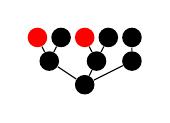
\begin{tikzpicture}[scale=.2]
\node[circle, scale=0.75, fill] (tid0) at (3.75,1.5){};
\node[circle, scale=0.75, fill] (tid1) at (1.5,3){};
\node[circle, scale=0.75, fill, red] (tid4) at (0.75,4.5){};
\node[circle, scale=0.75, fill] (tid5) at (2.25,4.5){};
\draw[](tid1) -- (tid4);
\draw[](tid1) -- (tid5);
\node[circle, scale=0.75, fill] (tid2) at (4.5,3){};
\node[circle, scale=0.75, fill, red] (tid6) at (3.75,4.5){};
\node[circle, scale=0.75, fill] (tid7) at (5.25,4.5){};
\draw[](tid2) -- (tid6);
\draw[](tid2) -- (tid7);
\node[circle, scale=0.75, fill] (tid3) at (6.75,3){};
\node[circle, scale=0.75, fill] (tid8) at (6.75,4.5){};
\draw[](tid3) -- (tid8);
\draw[](tid0) -- (tid1);
\draw[](tid0) -- (tid2);
\draw[](tid0) -- (tid3);
\end{tikzpicture}
\nodepart{two}
\footnotesize{5.625}
\nodepart{three}
\footnotesize{$67\:33$}
};
\node[draw opacity=0, fill opacity=0, anchor=south west] (dummyL) at (-15, -30){};
\node[draw=black, rectangle split, anchor=south west, rectangle split parts=3] (sn0x2611eb0) at ([xshift=2cm]sn0x261e5f0.south east){
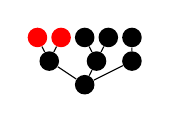
\begin{tikzpicture}[scale=.2]
\node[circle, scale=0.75, fill] (tid0) at (3.75,1.5){};
\node[circle, scale=0.75, fill] (tid1) at (1.5,3){};
\node[circle, scale=0.75, fill, red] (tid4) at (0.75,4.5){};
\node[circle, scale=0.75, fill, red] (tid5) at (2.25,4.5){};
\draw[](tid1) -- (tid4);
\draw[](tid1) -- (tid5);
\node[circle, scale=0.75, fill] (tid2) at (4.5,3){};
\node[circle, scale=0.75, fill] (tid6) at (3.75,4.5){};
\node[circle, scale=0.75, fill] (tid7) at (5.25,4.5){};
\draw[](tid2) -- (tid6);
\draw[](tid2) -- (tid7);
\node[circle, scale=0.75, fill] (tid3) at (6.75,3){};
\node[circle, scale=0.75, fill] (tid8) at (6.75,4.5){};
\draw[](tid3) -- (tid8);
\draw[](tid0) -- (tid1);
\draw[](tid0) -- (tid2);
\draw[](tid0) -- (tid3);
\end{tikzpicture}
\nodepart{two}
\footnotesize{5.625}
\nodepart{three}
\footnotesize{$67\:33$}
};
\node[draw opacity=0, fill opacity=0, anchor=south west] (dummyL) at (-15, -30){};
\node[draw=black, rectangle split, anchor=south west, rectangle split parts=3] (sn0x26163b0) at ([xshift=2cm]sn0x2611eb0.south east){
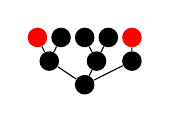
\begin{tikzpicture}[scale=.2]
\node[circle, scale=0.75, fill] (tid0) at (3.75,1.5){};
\node[circle, scale=0.75, fill] (tid1) at (1.5,3){};
\node[circle, scale=0.75, fill, red] (tid4) at (0.75,4.5){};
\node[circle, scale=0.75, fill] (tid5) at (2.25,4.5){};
\draw[](tid1) -- (tid4);
\draw[](tid1) -- (tid5);
\node[circle, scale=0.75, fill] (tid2) at (4.5,3){};
\node[circle, scale=0.75, fill] (tid6) at (3.75,4.5){};
\node[circle, scale=0.75, fill] (tid7) at (5.25,4.5){};
\draw[](tid2) -- (tid6);
\draw[](tid2) -- (tid7);
\node[circle, scale=0.75, fill] (tid3) at (6.75,3){};
\node[circle, scale=0.75, fill, red] (tid8) at (6.75,4.5){};
\draw[](tid3) -- (tid8);
\draw[](tid0) -- (tid1);
\draw[](tid0) -- (tid2);
\draw[](tid0) -- (tid3);
\end{tikzpicture}
\nodepart{two}
\footnotesize{5.625}
\nodepart{three}
\footnotesize{$33\:17\:17\:33$}
};
\node[draw opacity=0, fill opacity=0, anchor=south west] (dummyL) at (-15, -30){};
\node[draw=black, rectangle split, anchor=south west, rectangle split parts=3] (sn0x2617080) at ([xshift=2cm]sn0x26163b0.south east){
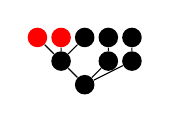
\begin{tikzpicture}[scale=.2]
\node[circle, scale=0.75, fill] (tid0) at (3.75,1.5){};
\node[circle, scale=0.75, fill] (tid1) at (2.25,3){};
\node[circle, scale=0.75, fill, red] (tid4) at (0.75,4.5){};
\node[circle, scale=0.75, fill, red] (tid5) at (2.25,4.5){};
\node[circle, scale=0.75, fill] (tid6) at (3.75,4.5){};
\draw[](tid1) -- (tid4);
\draw[](tid1) -- (tid5);
\draw[](tid1) -- (tid6);
\node[circle, scale=0.75, fill] (tid2) at (5.25,3){};
\node[circle, scale=0.75, fill] (tid7) at (5.25,4.5){};
\draw[](tid2) -- (tid7);
\node[circle, scale=0.75, fill] (tid3) at (6.75,3){};
\node[circle, scale=0.75, fill] (tid8) at (6.75,4.5){};
\draw[](tid3) -- (tid8);
\draw[](tid0) -- (tid1);
\draw[](tid0) -- (tid2);
\draw[](tid0) -- (tid3);
\end{tikzpicture}
\nodepart{two}
\footnotesize{5.625}
\nodepart{three}
\footnotesize{$67\:33$}
};
\node[draw opacity=0, fill opacity=0, anchor=south west] (dummyL) at (-15, -30){};
\node[draw=black, rectangle split, anchor=south west, rectangle split parts=3] (sn0x26126f0) at ([xshift=2cm]sn0x2617080.south east){
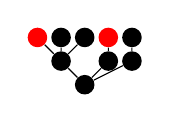
\begin{tikzpicture}[scale=.2]
\node[circle, scale=0.75, fill] (tid0) at (3.75,1.5){};
\node[circle, scale=0.75, fill] (tid1) at (2.25,3){};
\node[circle, scale=0.75, fill, red] (tid4) at (0.75,4.5){};
\node[circle, scale=0.75, fill] (tid5) at (2.25,4.5){};
\node[circle, scale=0.75, fill] (tid6) at (3.75,4.5){};
\draw[](tid1) -- (tid4);
\draw[](tid1) -- (tid5);
\draw[](tid1) -- (tid6);
\node[circle, scale=0.75, fill] (tid2) at (5.25,3){};
\node[circle, scale=0.75, fill, red] (tid7) at (5.25,4.5){};
\draw[](tid2) -- (tid7);
\node[circle, scale=0.75, fill] (tid3) at (6.75,3){};
\node[circle, scale=0.75, fill] (tid8) at (6.75,4.5){};
\draw[](tid3) -- (tid8);
\draw[](tid0) -- (tid1);
\draw[](tid0) -- (tid2);
\draw[](tid0) -- (tid3);
\end{tikzpicture}
\nodepart{two}
\footnotesize{5.625}
\nodepart{three}
\footnotesize{$33\:17\:33\:17$}
};
\node[draw opacity=0, fill opacity=0, anchor=south west] (dummyL) at (-21, -45){};
\node[draw=black, rectangle split, anchor=south west, rectangle split parts=3] (sn0x2612000) at ([xshift=2cm]dummyL){
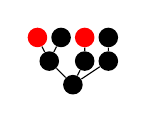
\begin{tikzpicture}[scale=.2]
\node[circle, scale=0.75, fill] (tid0) at (3,1.5){};
\node[circle, scale=0.75, fill] (tid1) at (1.5,3){};
\node[circle, scale=0.75, fill, red] (tid4) at (0.75,4.5){};
\node[circle, scale=0.75, fill] (tid5) at (2.25,4.5){};
\draw[](tid1) -- (tid4);
\draw[](tid1) -- (tid5);
\node[circle, scale=0.75, fill] (tid2) at (3.75,3){};
\node[circle, scale=0.75, fill, red] (tid6) at (3.75,4.5){};
\draw[](tid2) -- (tid6);
\node[circle, scale=0.75, fill] (tid3) at (5.25,3){};
\node[circle, scale=0.75, fill] (tid7) at (5.25,4.5){};
\draw[](tid3) -- (tid7);
\draw[](tid0) -- (tid1);
\draw[](tid0) -- (tid2);
\draw[](tid0) -- (tid3);
\end{tikzpicture}
\nodepart{two}
\footnotesize{5.125}
\nodepart{three}
\footnotesize{$50\:25\:25$}
};
\node[draw opacity=0, fill opacity=0, anchor=south west] (dummyL) at (-21, -45){};
\node[draw=black, rectangle split, anchor=south west, rectangle split parts=3] (sn0x2615a00) at ([xshift=2cm]sn0x2612000.south east){
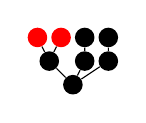
\begin{tikzpicture}[scale=.2]
\node[circle, scale=0.75, fill] (tid0) at (3,1.5){};
\node[circle, scale=0.75, fill] (tid1) at (1.5,3){};
\node[circle, scale=0.75, fill, red] (tid4) at (0.75,4.5){};
\node[circle, scale=0.75, fill, red] (tid5) at (2.25,4.5){};
\draw[](tid1) -- (tid4);
\draw[](tid1) -- (tid5);
\node[circle, scale=0.75, fill] (tid2) at (3.75,3){};
\node[circle, scale=0.75, fill] (tid6) at (3.75,4.5){};
\draw[](tid2) -- (tid6);
\node[circle, scale=0.75, fill] (tid3) at (5.25,3){};
\node[circle, scale=0.75, fill] (tid7) at (5.25,4.5){};
\draw[](tid3) -- (tid7);
\draw[](tid0) -- (tid1);
\draw[](tid0) -- (tid2);
\draw[](tid0) -- (tid3);
\end{tikzpicture}
\nodepart{two}
\footnotesize{5.125}
\nodepart{three}
\footnotesize{$1$}
};
\node[draw opacity=0, fill opacity=0, anchor=south west] (dummyL) at (-21, -45){};
\node[draw=black, rectangle split, anchor=south west, rectangle split parts=3] (sn0x26212b0) at ([xshift=2cm]sn0x2615a00.south east){
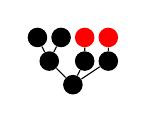
\begin{tikzpicture}[scale=.2]
\node[circle, scale=0.75, fill] (tid0) at (3,1.5){};
\node[circle, scale=0.75, fill] (tid1) at (1.5,3){};
\node[circle, scale=0.75, fill] (tid4) at (0.75,4.5){};
\node[circle, scale=0.75, fill] (tid5) at (2.25,4.5){};
\draw[](tid1) -- (tid4);
\draw[](tid1) -- (tid5);
\node[circle, scale=0.75, fill] (tid2) at (3.75,3){};
\node[circle, scale=0.75, fill, red] (tid6) at (3.75,4.5){};
\draw[](tid2) -- (tid6);
\node[circle, scale=0.75, fill] (tid3) at (5.25,3){};
\node[circle, scale=0.75, fill, red] (tid7) at (5.25,4.5){};
\draw[](tid3) -- (tid7);
\draw[](tid0) -- (tid1);
\draw[](tid0) -- (tid2);
\draw[](tid0) -- (tid3);
\end{tikzpicture}
\nodepart{two}
\footnotesize{5.125}
\nodepart{three}
\footnotesize{$1$}
};
\node[draw opacity=0, fill opacity=0, anchor=south west] (dummyL) at (-21, -45){};
\node[draw=black, rectangle split, anchor=south west, rectangle split parts=3] (sn0x2621ec0) at ([xshift=2cm]sn0x26212b0.south east){
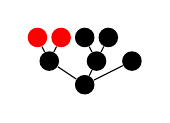
\begin{tikzpicture}[scale=.2]
\node[circle, scale=0.75, fill] (tid0) at (3.75,1.5){};
\node[circle, scale=0.75, fill] (tid1) at (1.5,3){};
\node[circle, scale=0.75, fill, red] (tid4) at (0.75,4.5){};
\node[circle, scale=0.75, fill, red] (tid5) at (2.25,4.5){};
\draw[](tid1) -- (tid4);
\draw[](tid1) -- (tid5);
\node[circle, scale=0.75, fill] (tid2) at (4.5,3){};
\node[circle, scale=0.75, fill] (tid6) at (3.75,4.5){};
\node[circle, scale=0.75, fill] (tid7) at (5.25,4.5){};
\draw[](tid2) -- (tid6);
\draw[](tid2) -- (tid7);
\node[circle, scale=0.75, fill] (tid3) at (6.75,3){};
\draw[](tid0) -- (tid1);
\draw[](tid0) -- (tid2);
\draw[](tid0) -- (tid3);
\end{tikzpicture}
\nodepart{two}
\footnotesize{5.125}
\nodepart{three}
\footnotesize{$1$}
};
\node[draw opacity=0, fill opacity=0, anchor=south west] (dummyL) at (-21, -45){};
\node[draw=black, rectangle split, anchor=south west, rectangle split parts=3] (sn0x26219b0) at ([xshift=2cm]sn0x2621ec0.south east){
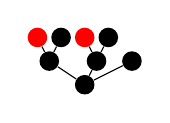
\begin{tikzpicture}[scale=.2]
\node[circle, scale=0.75, fill] (tid0) at (3.75,1.5){};
\node[circle, scale=0.75, fill] (tid1) at (1.5,3){};
\node[circle, scale=0.75, fill, red] (tid4) at (0.75,4.5){};
\node[circle, scale=0.75, fill] (tid5) at (2.25,4.5){};
\draw[](tid1) -- (tid4);
\draw[](tid1) -- (tid5);
\node[circle, scale=0.75, fill] (tid2) at (4.5,3){};
\node[circle, scale=0.75, fill, red] (tid6) at (3.75,4.5){};
\node[circle, scale=0.75, fill] (tid7) at (5.25,4.5){};
\draw[](tid2) -- (tid6);
\draw[](tid2) -- (tid7);
\node[circle, scale=0.75, fill] (tid3) at (6.75,3){};
\draw[](tid0) -- (tid1);
\draw[](tid0) -- (tid2);
\draw[](tid0) -- (tid3);
\end{tikzpicture}
\nodepart{two}
\footnotesize{5.125}
\nodepart{three}
\footnotesize{$50\:50$}
};
\node[draw opacity=0, fill opacity=0, anchor=south west] (dummyL) at (-21, -45){};
\node[draw=black, rectangle split, anchor=south west, rectangle split parts=3] (sn0x2622820) at ([xshift=2cm]sn0x26219b0.south east){
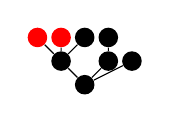
\begin{tikzpicture}[scale=.2]
\node[circle, scale=0.75, fill] (tid0) at (3.75,1.5){};
\node[circle, scale=0.75, fill] (tid1) at (2.25,3){};
\node[circle, scale=0.75, fill, red] (tid4) at (0.75,4.5){};
\node[circle, scale=0.75, fill, red] (tid5) at (2.25,4.5){};
\node[circle, scale=0.75, fill] (tid6) at (3.75,4.5){};
\draw[](tid1) -- (tid4);
\draw[](tid1) -- (tid5);
\draw[](tid1) -- (tid6);
\node[circle, scale=0.75, fill] (tid2) at (5.25,3){};
\node[circle, scale=0.75, fill] (tid7) at (5.25,4.5){};
\draw[](tid2) -- (tid7);
\node[circle, scale=0.75, fill] (tid3) at (6.75,3){};
\draw[](tid0) -- (tid1);
\draw[](tid0) -- (tid2);
\draw[](tid0) -- (tid3);
\end{tikzpicture}
\nodepart{two}
\footnotesize{5.125}
\nodepart{three}
\footnotesize{$50\:50$}
};
\node[draw opacity=0, fill opacity=0, anchor=south west] (dummyL) at (-21, -45){};
\node[draw=black, rectangle split, anchor=south west, rectangle split parts=3] (sn0x2622950) at ([xshift=2cm]sn0x2622820.south east){
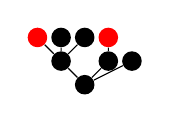
\begin{tikzpicture}[scale=.2]
\node[circle, scale=0.75, fill] (tid0) at (3.75,1.5){};
\node[circle, scale=0.75, fill] (tid1) at (2.25,3){};
\node[circle, scale=0.75, fill, red] (tid4) at (0.75,4.5){};
\node[circle, scale=0.75, fill] (tid5) at (2.25,4.5){};
\node[circle, scale=0.75, fill] (tid6) at (3.75,4.5){};
\draw[](tid1) -- (tid4);
\draw[](tid1) -- (tid5);
\draw[](tid1) -- (tid6);
\node[circle, scale=0.75, fill] (tid2) at (5.25,3){};
\node[circle, scale=0.75, fill, red] (tid7) at (5.25,4.5){};
\draw[](tid2) -- (tid7);
\node[circle, scale=0.75, fill] (tid3) at (6.75,3){};
\draw[](tid0) -- (tid1);
\draw[](tid0) -- (tid2);
\draw[](tid0) -- (tid3);
\end{tikzpicture}
\nodepart{two}
\footnotesize{5.125}
\nodepart{three}
\footnotesize{$50\:50$}
};
\node[draw opacity=0, fill opacity=0, anchor=south west] (dummyL) at (-12, -60){};
\node[draw=black, rectangle split, anchor=south west, rectangle split parts=3] (sn0x2614f90) at ([xshift=2cm]dummyL){
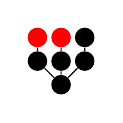
\begin{tikzpicture}[scale=.2]
\node[circle, scale=0.75, fill] (tid0) at (2.25,1.5){};
\node[circle, scale=0.75, fill] (tid1) at (0.75,3){};
\node[circle, scale=0.75, fill, red] (tid4) at (0.75,4.5){};
\draw[](tid1) -- (tid4);
\node[circle, scale=0.75, fill] (tid2) at (2.25,3){};
\node[circle, scale=0.75, fill, red] (tid5) at (2.25,4.5){};
\draw[](tid2) -- (tid5);
\node[circle, scale=0.75, fill] (tid3) at (3.75,3){};
\node[circle, scale=0.75, fill] (tid6) at (3.75,4.5){};
\draw[](tid3) -- (tid6);
\draw[](tid0) -- (tid1);
\draw[](tid0) -- (tid2);
\draw[](tid0) -- (tid3);
\end{tikzpicture}
\nodepart{two}
\footnotesize{4.625}
\nodepart{three}
\footnotesize{$1$}
};
\node[draw opacity=0, fill opacity=0, anchor=south west] (dummyL) at (-12, -60){};
\node[draw=black, rectangle split, anchor=south west, rectangle split parts=3] (sn0x261e6b0) at ([xshift=2cm]sn0x2614f90.south east){
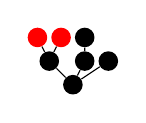
\begin{tikzpicture}[scale=.2]
\node[circle, scale=0.75, fill] (tid0) at (3,1.5){};
\node[circle, scale=0.75, fill] (tid1) at (1.5,3){};
\node[circle, scale=0.75, fill, red] (tid4) at (0.75,4.5){};
\node[circle, scale=0.75, fill, red] (tid5) at (2.25,4.5){};
\draw[](tid1) -- (tid4);
\draw[](tid1) -- (tid5);
\node[circle, scale=0.75, fill] (tid2) at (3.75,3){};
\node[circle, scale=0.75, fill] (tid6) at (3.75,4.5){};
\draw[](tid2) -- (tid6);
\node[circle, scale=0.75, fill] (tid3) at (5.25,3){};
\draw[](tid0) -- (tid1);
\draw[](tid0) -- (tid2);
\draw[](tid0) -- (tid3);
\end{tikzpicture}
\nodepart{two}
\footnotesize{4.625}
\nodepart{three}
\footnotesize{$1$}
};
\node[draw opacity=0, fill opacity=0, anchor=south west] (dummyL) at (-12, -60){};
\node[draw=black, rectangle split, anchor=south west, rectangle split parts=3] (sn0x261f7a0) at ([xshift=2cm]sn0x261e6b0.south east){
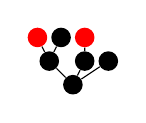
\begin{tikzpicture}[scale=.2]
\node[circle, scale=0.75, fill] (tid0) at (3,1.5){};
\node[circle, scale=0.75, fill] (tid1) at (1.5,3){};
\node[circle, scale=0.75, fill, red] (tid4) at (0.75,4.5){};
\node[circle, scale=0.75, fill] (tid5) at (2.25,4.5){};
\draw[](tid1) -- (tid4);
\draw[](tid1) -- (tid5);
\node[circle, scale=0.75, fill] (tid2) at (3.75,3){};
\node[circle, scale=0.75, fill, red] (tid6) at (3.75,4.5){};
\draw[](tid2) -- (tid6);
\node[circle, scale=0.75, fill] (tid3) at (5.25,3){};
\draw[](tid0) -- (tid1);
\draw[](tid0) -- (tid2);
\draw[](tid0) -- (tid3);
\end{tikzpicture}
\nodepart{two}
\footnotesize{4.625}
\nodepart{three}
\footnotesize{$50\:50$}
};
\node[draw opacity=0, fill opacity=0, anchor=south west] (dummyL) at (-12, -60){};
\node[draw=black, rectangle split, anchor=south west, rectangle split parts=3] (sn0x26232c0) at ([xshift=2cm]sn0x261f7a0.south east){
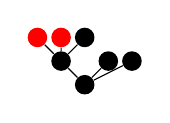
\begin{tikzpicture}[scale=.2]
\node[circle, scale=0.75, fill] (tid0) at (3.75,1.5){};
\node[circle, scale=0.75, fill] (tid1) at (2.25,3){};
\node[circle, scale=0.75, fill, red] (tid4) at (0.75,4.5){};
\node[circle, scale=0.75, fill, red] (tid5) at (2.25,4.5){};
\node[circle, scale=0.75, fill] (tid6) at (3.75,4.5){};
\draw[](tid1) -- (tid4);
\draw[](tid1) -- (tid5);
\draw[](tid1) -- (tid6);
\node[circle, scale=0.75, fill] (tid2) at (5.25,3){};
\node[circle, scale=0.75, fill] (tid3) at (6.75,3){};
\draw[](tid0) -- (tid1);
\draw[](tid0) -- (tid2);
\draw[](tid0) -- (tid3);
\end{tikzpicture}
\nodepart{two}
\footnotesize{4.625}
\nodepart{three}
\footnotesize{$1$}
};
\node[draw opacity=0, fill opacity=0, anchor=south west] (dummyL) at (-6, -75){};
\node[draw=black, rectangle split, anchor=south west, rectangle split parts=3] (sn0x261fa80) at ([xshift=2cm]dummyL){
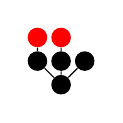
\begin{tikzpicture}[scale=.2]
\node[circle, scale=0.75, fill] (tid0) at (2.25,1.5){};
\node[circle, scale=0.75, fill] (tid1) at (0.75,3){};
\node[circle, scale=0.75, fill, red] (tid4) at (0.75,4.5){};
\draw[](tid1) -- (tid4);
\node[circle, scale=0.75, fill] (tid2) at (2.25,3){};
\node[circle, scale=0.75, fill, red] (tid5) at (2.25,4.5){};
\draw[](tid2) -- (tid5);
\node[circle, scale=0.75, fill] (tid3) at (3.75,3){};
\draw[](tid0) -- (tid1);
\draw[](tid0) -- (tid2);
\draw[](tid0) -- (tid3);
\end{tikzpicture}
\nodepart{two}
\footnotesize{4.125}
\nodepart{three}
\footnotesize{$1$}
};
\node[draw opacity=0, fill opacity=0, anchor=south west] (dummyL) at (-6, -75){};
\node[draw=black, rectangle split, anchor=south west, rectangle split parts=3] (sn0x2620400) at ([xshift=2cm]sn0x261fa80.south east){
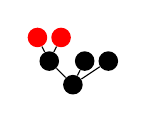
\begin{tikzpicture}[scale=.2]
\node[circle, scale=0.75, fill] (tid0) at (3,1.5){};
\node[circle, scale=0.75, fill] (tid1) at (1.5,3){};
\node[circle, scale=0.75, fill, red] (tid4) at (0.75,4.5){};
\node[circle, scale=0.75, fill, red] (tid5) at (2.25,4.5){};
\draw[](tid1) -- (tid4);
\draw[](tid1) -- (tid5);
\node[circle, scale=0.75, fill] (tid2) at (3.75,3){};
\node[circle, scale=0.75, fill] (tid3) at (5.25,3){};
\draw[](tid0) -- (tid1);
\draw[](tid0) -- (tid2);
\draw[](tid0) -- (tid3);
\end{tikzpicture}
\nodepart{two}
\footnotesize{4.125}
\nodepart{three}
\footnotesize{$1$}
};
\node[draw opacity=0, fill opacity=0, anchor=south west] (dummyL) at (-3, -90){};
\node[draw=black, rectangle split, anchor=south west, rectangle split parts=3] (sn0x261fb40) at ([xshift=2cm]dummyL){
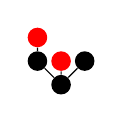
\begin{tikzpicture}[scale=.2]
\node[circle, scale=0.75, fill] (tid0) at (2.25,1.5){};
\node[circle, scale=0.75, fill] (tid1) at (0.75,3){};
\node[circle, scale=0.75, fill, red] (tid4) at (0.75,4.5){};
\draw[](tid1) -- (tid4);
\node[circle, scale=0.75, fill, red] (tid2) at (2.25,3){};
\node[circle, scale=0.75, fill] (tid3) at (3.75,3){};
\draw[](tid0) -- (tid1);
\draw[](tid0) -- (tid2);
\draw[](tid0) -- (tid3);
\end{tikzpicture}
\nodepart{two}
\footnotesize{3.625}
\nodepart{three}
\footnotesize{$50\:50$}
};
\node[draw opacity=0, fill opacity=0, anchor=south west] (dummyL) at (-6, -105){};
\node[draw=black, rectangle split, anchor=south west, rectangle split parts=3] (sn0x261f8e0) at ([xshift=2cm]dummyL){
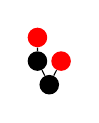
\begin{tikzpicture}[scale=.2]
\node[circle, scale=0.75, fill] (tid0) at (1.5,1.5){};
\node[circle, scale=0.75, fill] (tid1) at (0.75,3){};
\node[circle, scale=0.75, fill, red] (tid3) at (0.75,4.5){};
\draw[](tid1) -- (tid3);
\node[circle, scale=0.75, fill, red] (tid2) at (2.25,3){};
\draw[](tid0) -- (tid1);
\draw[](tid0) -- (tid2);
\end{tikzpicture}
\nodepart{two}
\footnotesize{3.25}
\nodepart{three}
\footnotesize{$50\:50$}
};
\node[draw opacity=0, fill opacity=0, anchor=south west] (dummyL) at (-6, -105){};
\node[draw=black, rectangle split, anchor=south west, rectangle split parts=3] (sn0x261fd90) at ([xshift=2cm]sn0x261f8e0.south east){
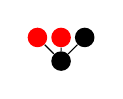
\begin{tikzpicture}[scale=.2]
\node[circle, scale=0.75, fill] (tid0) at (2.25,1.5){};
\node[circle, scale=0.75, fill, red] (tid1) at (0.75,3){};
\node[circle, scale=0.75, fill, red] (tid2) at (2.25,3){};
\node[circle, scale=0.75, fill] (tid3) at (3.75,3){};
\draw[](tid0) -- (tid1);
\draw[](tid0) -- (tid2);
\draw[](tid0) -- (tid3);
\end{tikzpicture}
\nodepart{two}
\footnotesize{3}
\nodepart{three}
\footnotesize{$1$}
};
\node[draw opacity=0, fill opacity=0, anchor=south west] (dummyL) at (-6, -120){};
\node[draw=black, rectangle split, anchor=south west, rectangle split parts=3] (sn0x261fe50) at ([xshift=2cm]dummyL){
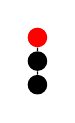
\begin{tikzpicture}[scale=.2]
\node[circle, scale=0.75, fill] (tid0) at (0.75,1.5){};
\node[circle, scale=0.75, fill] (tid1) at (0.75,3){};
\node[circle, scale=0.75, fill, red] (tid2) at (0.75,4.5){};
\draw[](tid1) -- (tid2);
\draw[](tid0) -- (tid1);
\end{tikzpicture}
\nodepart{two}
\footnotesize{3}
\nodepart{three}
\footnotesize{$1$}
};
\node[draw opacity=0, fill opacity=0, anchor=south west] (dummyL) at (-6, -120){};
\node[draw=black, rectangle split, anchor=south west, rectangle split parts=3] (sn0x261ff10) at ([xshift=2cm]sn0x261fe50.south east){

\begin{tikzpicture}[scale=.2]
\node[circle, scale=0.75, fill] (tid0) at (1.5,1.5){};
\node[circle, scale=0.75, fill, red] (tid1) at (0.75,3){};
\node[circle, scale=0.75, fill, red] (tid2) at (2.25,3){};
\draw[](tid0) -- (tid1);
\draw[](tid0) -- (tid2);
\end{tikzpicture}
\nodepart{two}
\footnotesize{2.5}
\nodepart{three}
\footnotesize{$1$}
};
\node[draw opacity=0, fill opacity=0, anchor=south west] (dummyL) at (-3, -135){};
\node[draw=black, rectangle split, anchor=south west, rectangle split parts=3] (sn0x2620120) at ([xshift=2cm]dummyL){

\begin{tikzpicture}[scale=.2]
\node[circle, scale=0.75, fill] (tid0) at (0.75,1.5){};
\node[circle, scale=0.75, fill, red] (tid1) at (0.75,3){};
\draw[](tid0) -- (tid1);
\end{tikzpicture}
\nodepart{two}
\footnotesize{2}
\nodepart{three}
\footnotesize{$1$}
};
\node[draw opacity=0, fill opacity=0, anchor=south west] (dummyL) at (-3, -150){};
\node[draw=black, rectangle split, anchor=south west, rectangle split parts=3] (sn0x26201e0) at ([xshift=2cm]dummyL){

\begin{tikzpicture}[scale=.2]
\node[circle, scale=0.75, fill, red] (tid0) at (0.75,1.5){};
\end{tikzpicture}
\nodepart{two}
\footnotesize{1}
\nodepart{three}
\footnotesize{$$}
};
\draw (sn0x26141c0.south) -- (sn0x261e5f0.north);
\draw (sn0x26141c0.south) -- (sn0x2611eb0.north);
\draw (sn0x26141c0.south) -- (sn0x26163b0.north);
\draw (sn0x26141c0.south) -- (sn0x2617080.north);
\draw (sn0x26141c0.south) -- (sn0x26126f0.north);
\draw (sn0x261e5f0.south) -- (sn0x2612000.north);
\draw (sn0x261e5f0.south) -- (sn0x2615a00.north);
\draw (sn0x2611eb0.south) -- (sn0x2612000.north);
\draw (sn0x2611eb0.south) -- (sn0x26212b0.north);
\draw (sn0x26163b0.south) -- (sn0x26212b0.north);
\draw (sn0x26163b0.south) -- (sn0x2612000.north);
\draw (sn0x26163b0.south) -- (sn0x2621ec0.north);
\draw (sn0x26163b0.south) -- (sn0x26219b0.north);
\draw (sn0x2617080.south) -- (sn0x2615a00.north);
\draw (sn0x2617080.south) -- (sn0x2612000.north);
\draw (sn0x26126f0.south) -- (sn0x2612000.north);
\draw (sn0x26126f0.south) -- (sn0x26212b0.north);
\draw (sn0x26126f0.south) -- (sn0x2622820.north);
\draw (sn0x26126f0.south) -- (sn0x2622950.north);
\draw (sn0x2612000.south) -- (sn0x2614f90.north);
\draw (sn0x2612000.south) -- (sn0x261e6b0.north);
\draw (sn0x2612000.south) -- (sn0x261f7a0.north);
\draw (sn0x2615a00.south) -- (sn0x2614f90.north);
\draw (sn0x26212b0.south) -- (sn0x261f7a0.north);
\draw (sn0x2621ec0.south) -- (sn0x261f7a0.north);
\draw (sn0x26219b0.south) -- (sn0x261f7a0.north);
\draw (sn0x26219b0.south) -- (sn0x261e6b0.north);
\draw (sn0x2622820.south) -- (sn0x261e6b0.north);
\draw (sn0x2622820.south) -- (sn0x261f7a0.north);
\draw (sn0x2622950.south) -- (sn0x261f7a0.north);
\draw (sn0x2622950.south) -- (sn0x26232c0.north);
\draw (sn0x2614f90.south) -- (sn0x261fa80.north);
\draw (sn0x261e6b0.south) -- (sn0x261fa80.north);
\draw (sn0x261f7a0.south) -- (sn0x261fa80.north);
\draw (sn0x261f7a0.south) -- (sn0x2620400.north);
\draw (sn0x26232c0.south) -- (sn0x2620400.north);
\draw (sn0x261fa80.south) -- (sn0x261fb40.north);
\draw (sn0x2620400.south) -- (sn0x261fb40.north);
\draw (sn0x261fb40.south) -- (sn0x261f8e0.north);
\draw (sn0x261fb40.south) -- (sn0x261fd90.north);
\draw (sn0x261f8e0.south) -- (sn0x261fe50.north);
\draw (sn0x261f8e0.south) -- (sn0x261ff10.north);
\draw (sn0x261fd90.south) -- (sn0x261ff10.north);
\draw (sn0x261fe50.south) -- (sn0x2620120.north);
\draw (sn0x261ff10.south) -- (sn0x2620120.north);
\draw (sn0x2620120.south) -- (sn0x26201e0.north);
\end{tikzpicture}

%%% Local Variables:
%%% TeX-master: "thesis/thesis.tex"
%%% End: 
\begin{tikzpicture}[scale=.2, anchor=west]
\node[draw opacity=0, fill opacity=0, anchor=south west] (dummyL) at (-3, -15){};
\node[draw=black, rectangle split, anchor=south west, rectangle split parts=3] (sn0x2614278) at ([xshift=2cm]dummyL){
\begin{tikzpicture}[scale=.2]
\node[circle, scale=0.75, fill] (tid0) at (4.5,1.5){};
\node[circle, scale=0.75, fill] (tid1) at (2.25,3){};
\node[circle, scale=0.75, fill, red] (tid4) at (0.75,4.5){};
\node[circle, scale=0.75, fill, red] (tid5) at (2.25,4.5){};
\node[circle, scale=0.75, fill] (tid6) at (3.75,4.5){};
\draw[](tid1) -- (tid4);
\draw[](tid1) -- (tid5);
\draw[](tid1) -- (tid6);
\node[circle, scale=0.75, fill] (tid2) at (6,3){};
\node[circle, scale=0.75, fill] (tid7) at (5.25,4.5){};
\node[circle, scale=0.75, fill] (tid8) at (6.75,4.5){};
\draw[](tid2) -- (tid7);
\draw[](tid2) -- (tid8);
\node[circle, scale=0.75, fill] (tid3) at (8.25,3){};
\node[circle, scale=0.75, fill] (tid9) at (8.25,4.5){};
\draw[](tid3) -- (tid9);
\draw[](tid0) -- (tid1);
\draw[](tid0) -- (tid2);
\draw[](tid0) -- (tid3);
\end{tikzpicture}
\nodepart{two}
\footnotesize{6.125}
\nodepart{three}
\footnotesize{$25\:50\:25$}
};
\node[draw opacity=0, fill opacity=0, anchor=south west] (dummyL) at (-9, -30){};
\node[draw=black, rectangle split, anchor=south west, rectangle split parts=3] (sn0x2611eb0) at ([xshift=2cm]dummyL){
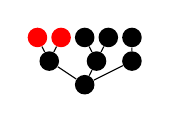
\begin{tikzpicture}[scale=.2]
\node[circle, scale=0.75, fill] (tid0) at (3.75,1.5){};
\node[circle, scale=0.75, fill] (tid1) at (1.5,3){};
\node[circle, scale=0.75, fill, red] (tid4) at (0.75,4.5){};
\node[circle, scale=0.75, fill, red] (tid5) at (2.25,4.5){};
\draw[](tid1) -- (tid4);
\draw[](tid1) -- (tid5);
\node[circle, scale=0.75, fill] (tid2) at (4.5,3){};
\node[circle, scale=0.75, fill] (tid6) at (3.75,4.5){};
\node[circle, scale=0.75, fill] (tid7) at (5.25,4.5){};
\draw[](tid2) -- (tid6);
\draw[](tid2) -- (tid7);
\node[circle, scale=0.75, fill] (tid3) at (6.75,3){};
\node[circle, scale=0.75, fill] (tid8) at (6.75,4.5){};
\draw[](tid3) -- (tid8);
\draw[](tid0) -- (tid1);
\draw[](tid0) -- (tid2);
\draw[](tid0) -- (tid3);
\end{tikzpicture}
\nodepart{two}
\footnotesize{5.625}
\nodepart{three}
\footnotesize{$67\:33$}
};
\node[draw opacity=0, fill opacity=0, anchor=south west] (dummyL) at (-9, -30){};
\node[draw=black, rectangle split, anchor=south west, rectangle split parts=3] (sn0x261e5f0) at ([xshift=2cm]sn0x2611eb0.south east){
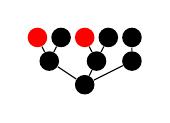
\begin{tikzpicture}[scale=.2]
\node[circle, scale=0.75, fill] (tid0) at (3.75,1.5){};
\node[circle, scale=0.75, fill] (tid1) at (1.5,3){};
\node[circle, scale=0.75, fill, red] (tid4) at (0.75,4.5){};
\node[circle, scale=0.75, fill] (tid5) at (2.25,4.5){};
\draw[](tid1) -- (tid4);
\draw[](tid1) -- (tid5);
\node[circle, scale=0.75, fill] (tid2) at (4.5,3){};
\node[circle, scale=0.75, fill, red] (tid6) at (3.75,4.5){};
\node[circle, scale=0.75, fill] (tid7) at (5.25,4.5){};
\draw[](tid2) -- (tid6);
\draw[](tid2) -- (tid7);
\node[circle, scale=0.75, fill] (tid3) at (6.75,3){};
\node[circle, scale=0.75, fill] (tid8) at (6.75,4.5){};
\draw[](tid3) -- (tid8);
\draw[](tid0) -- (tid1);
\draw[](tid0) -- (tid2);
\draw[](tid0) -- (tid3);
\end{tikzpicture}
\nodepart{two}
\footnotesize{5.625}
\nodepart{three}
\footnotesize{$67\:33$}
};
\node[draw opacity=0, fill opacity=0, anchor=south west] (dummyL) at (-9, -30){};
\node[draw=black, rectangle split, anchor=south west, rectangle split parts=3] (sn0x26163b0) at ([xshift=2cm]sn0x261e5f0.south east){
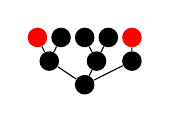
\begin{tikzpicture}[scale=.2]
\node[circle, scale=0.75, fill] (tid0) at (3.75,1.5){};
\node[circle, scale=0.75, fill] (tid1) at (1.5,3){};
\node[circle, scale=0.75, fill, red] (tid4) at (0.75,4.5){};
\node[circle, scale=0.75, fill] (tid5) at (2.25,4.5){};
\draw[](tid1) -- (tid4);
\draw[](tid1) -- (tid5);
\node[circle, scale=0.75, fill] (tid2) at (4.5,3){};
\node[circle, scale=0.75, fill] (tid6) at (3.75,4.5){};
\node[circle, scale=0.75, fill] (tid7) at (5.25,4.5){};
\draw[](tid2) -- (tid6);
\draw[](tid2) -- (tid7);
\node[circle, scale=0.75, fill] (tid3) at (6.75,3){};
\node[circle, scale=0.75, fill, red] (tid8) at (6.75,4.5){};
\draw[](tid3) -- (tid8);
\draw[](tid0) -- (tid1);
\draw[](tid0) -- (tid2);
\draw[](tid0) -- (tid3);
\end{tikzpicture}
\nodepart{two}
\footnotesize{5.625}
\nodepart{three}
\footnotesize{$33\:17\:17\:33$}
};
\node[draw opacity=0, fill opacity=0, anchor=south west] (dummyL) at (-15, -45){};
\node[draw=black, rectangle split, anchor=south west, rectangle split parts=3] (sn0x2612000) at ([xshift=2cm]dummyL){
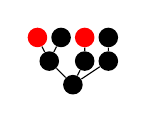
\begin{tikzpicture}[scale=.2]
\node[circle, scale=0.75, fill] (tid0) at (3,1.5){};
\node[circle, scale=0.75, fill] (tid1) at (1.5,3){};
\node[circle, scale=0.75, fill, red] (tid4) at (0.75,4.5){};
\node[circle, scale=0.75, fill] (tid5) at (2.25,4.5){};
\draw[](tid1) -- (tid4);
\draw[](tid1) -- (tid5);
\node[circle, scale=0.75, fill] (tid2) at (3.75,3){};
\node[circle, scale=0.75, fill, red] (tid6) at (3.75,4.5){};
\draw[](tid2) -- (tid6);
\node[circle, scale=0.75, fill] (tid3) at (5.25,3){};
\node[circle, scale=0.75, fill] (tid7) at (5.25,4.5){};
\draw[](tid3) -- (tid7);
\draw[](tid0) -- (tid1);
\draw[](tid0) -- (tid2);
\draw[](tid0) -- (tid3);
\end{tikzpicture}
\nodepart{two}
\footnotesize{5.125}
\nodepart{three}
\footnotesize{$50\:25\:25$}
};
\node[draw opacity=0, fill opacity=0, anchor=south west] (dummyL) at (-15, -45){};
\node[draw=black, rectangle split, anchor=south west, rectangle split parts=3] (sn0x26212b0) at ([xshift=2cm]sn0x2612000.south east){
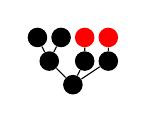
\begin{tikzpicture}[scale=.2]
\node[circle, scale=0.75, fill] (tid0) at (3,1.5){};
\node[circle, scale=0.75, fill] (tid1) at (1.5,3){};
\node[circle, scale=0.75, fill] (tid4) at (0.75,4.5){};
\node[circle, scale=0.75, fill] (tid5) at (2.25,4.5){};
\draw[](tid1) -- (tid4);
\draw[](tid1) -- (tid5);
\node[circle, scale=0.75, fill] (tid2) at (3.75,3){};
\node[circle, scale=0.75, fill, red] (tid6) at (3.75,4.5){};
\draw[](tid2) -- (tid6);
\node[circle, scale=0.75, fill] (tid3) at (5.25,3){};
\node[circle, scale=0.75, fill, red] (tid7) at (5.25,4.5){};
\draw[](tid3) -- (tid7);
\draw[](tid0) -- (tid1);
\draw[](tid0) -- (tid2);
\draw[](tid0) -- (tid3);
\end{tikzpicture}
\nodepart{two}
\footnotesize{5.125}
\nodepart{three}
\footnotesize{$1$}
};
\node[draw opacity=0, fill opacity=0, anchor=south west] (dummyL) at (-15, -45){};
\node[draw=black, rectangle split, anchor=south west, rectangle split parts=3] (sn0x2615a00) at ([xshift=2cm]sn0x26212b0.south east){
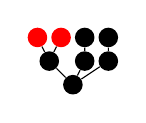
\begin{tikzpicture}[scale=.2]
\node[circle, scale=0.75, fill] (tid0) at (3,1.5){};
\node[circle, scale=0.75, fill] (tid1) at (1.5,3){};
\node[circle, scale=0.75, fill, red] (tid4) at (0.75,4.5){};
\node[circle, scale=0.75, fill, red] (tid5) at (2.25,4.5){};
\draw[](tid1) -- (tid4);
\draw[](tid1) -- (tid5);
\node[circle, scale=0.75, fill] (tid2) at (3.75,3){};
\node[circle, scale=0.75, fill] (tid6) at (3.75,4.5){};
\draw[](tid2) -- (tid6);
\node[circle, scale=0.75, fill] (tid3) at (5.25,3){};
\node[circle, scale=0.75, fill] (tid7) at (5.25,4.5){};
\draw[](tid3) -- (tid7);
\draw[](tid0) -- (tid1);
\draw[](tid0) -- (tid2);
\draw[](tid0) -- (tid3);
\end{tikzpicture}
\nodepart{two}
\footnotesize{5.125}
\nodepart{three}
\footnotesize{$1$}
};
\node[draw opacity=0, fill opacity=0, anchor=south west] (dummyL) at (-15, -45){};
\node[draw=black, rectangle split, anchor=south west, rectangle split parts=3] (sn0x2621ec0) at ([xshift=2cm]sn0x2615a00.south east){
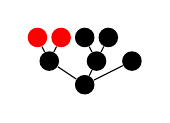
\begin{tikzpicture}[scale=.2]
\node[circle, scale=0.75, fill] (tid0) at (3.75,1.5){};
\node[circle, scale=0.75, fill] (tid1) at (1.5,3){};
\node[circle, scale=0.75, fill, red] (tid4) at (0.75,4.5){};
\node[circle, scale=0.75, fill, red] (tid5) at (2.25,4.5){};
\draw[](tid1) -- (tid4);
\draw[](tid1) -- (tid5);
\node[circle, scale=0.75, fill] (tid2) at (4.5,3){};
\node[circle, scale=0.75, fill] (tid6) at (3.75,4.5){};
\node[circle, scale=0.75, fill] (tid7) at (5.25,4.5){};
\draw[](tid2) -- (tid6);
\draw[](tid2) -- (tid7);
\node[circle, scale=0.75, fill] (tid3) at (6.75,3){};
\draw[](tid0) -- (tid1);
\draw[](tid0) -- (tid2);
\draw[](tid0) -- (tid3);
\end{tikzpicture}
\nodepart{two}
\footnotesize{5.125}
\nodepart{three}
\footnotesize{$1$}
};
\node[draw opacity=0, fill opacity=0, anchor=south west] (dummyL) at (-15, -45){};
\node[draw=black, rectangle split, anchor=south west, rectangle split parts=3] (sn0x26219b0) at ([xshift=2cm]sn0x2621ec0.south east){
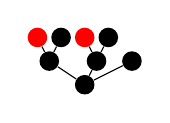
\begin{tikzpicture}[scale=.2]
\node[circle, scale=0.75, fill] (tid0) at (3.75,1.5){};
\node[circle, scale=0.75, fill] (tid1) at (1.5,3){};
\node[circle, scale=0.75, fill, red] (tid4) at (0.75,4.5){};
\node[circle, scale=0.75, fill] (tid5) at (2.25,4.5){};
\draw[](tid1) -- (tid4);
\draw[](tid1) -- (tid5);
\node[circle, scale=0.75, fill] (tid2) at (4.5,3){};
\node[circle, scale=0.75, fill, red] (tid6) at (3.75,4.5){};
\node[circle, scale=0.75, fill] (tid7) at (5.25,4.5){};
\draw[](tid2) -- (tid6);
\draw[](tid2) -- (tid7);
\node[circle, scale=0.75, fill] (tid3) at (6.75,3){};
\draw[](tid0) -- (tid1);
\draw[](tid0) -- (tid2);
\draw[](tid0) -- (tid3);
\end{tikzpicture}
\nodepart{two}
\footnotesize{5.125}
\nodepart{three}
\footnotesize{$50\:50$}
};
\node[draw opacity=0, fill opacity=0, anchor=south west] (dummyL) at (-9, -60){};
\node[draw=black, rectangle split, anchor=south west, rectangle split parts=3] (sn0x2614f90) at ([xshift=2cm]dummyL){
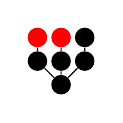
\begin{tikzpicture}[scale=.2]
\node[circle, scale=0.75, fill] (tid0) at (2.25,1.5){};
\node[circle, scale=0.75, fill] (tid1) at (0.75,3){};
\node[circle, scale=0.75, fill, red] (tid4) at (0.75,4.5){};
\draw[](tid1) -- (tid4);
\node[circle, scale=0.75, fill] (tid2) at (2.25,3){};
\node[circle, scale=0.75, fill, red] (tid5) at (2.25,4.5){};
\draw[](tid2) -- (tid5);
\node[circle, scale=0.75, fill] (tid3) at (3.75,3){};
\node[circle, scale=0.75, fill] (tid6) at (3.75,4.5){};
\draw[](tid3) -- (tid6);
\draw[](tid0) -- (tid1);
\draw[](tid0) -- (tid2);
\draw[](tid0) -- (tid3);
\end{tikzpicture}
\nodepart{two}
\footnotesize{4.625}
\nodepart{three}
\footnotesize{$1$}
};
\node[draw opacity=0, fill opacity=0, anchor=south west] (dummyL) at (-9, -60){};
\node[draw=black, rectangle split, anchor=south west, rectangle split parts=3] (sn0x261e6b0) at ([xshift=2cm]sn0x2614f90.south east){
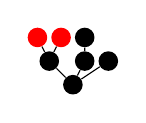
\begin{tikzpicture}[scale=.2]
\node[circle, scale=0.75, fill] (tid0) at (3,1.5){};
\node[circle, scale=0.75, fill] (tid1) at (1.5,3){};
\node[circle, scale=0.75, fill, red] (tid4) at (0.75,4.5){};
\node[circle, scale=0.75, fill, red] (tid5) at (2.25,4.5){};
\draw[](tid1) -- (tid4);
\draw[](tid1) -- (tid5);
\node[circle, scale=0.75, fill] (tid2) at (3.75,3){};
\node[circle, scale=0.75, fill] (tid6) at (3.75,4.5){};
\draw[](tid2) -- (tid6);
\node[circle, scale=0.75, fill] (tid3) at (5.25,3){};
\draw[](tid0) -- (tid1);
\draw[](tid0) -- (tid2);
\draw[](tid0) -- (tid3);
\end{tikzpicture}
\nodepart{two}
\footnotesize{4.625}
\nodepart{three}
\footnotesize{$1$}
};
\node[draw opacity=0, fill opacity=0, anchor=south west] (dummyL) at (-9, -60){};
\node[draw=black, rectangle split, anchor=south west, rectangle split parts=3] (sn0x261f7a0) at ([xshift=2cm]sn0x261e6b0.south east){
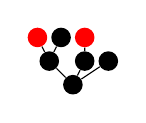
\begin{tikzpicture}[scale=.2]
\node[circle, scale=0.75, fill] (tid0) at (3,1.5){};
\node[circle, scale=0.75, fill] (tid1) at (1.5,3){};
\node[circle, scale=0.75, fill, red] (tid4) at (0.75,4.5){};
\node[circle, scale=0.75, fill] (tid5) at (2.25,4.5){};
\draw[](tid1) -- (tid4);
\draw[](tid1) -- (tid5);
\node[circle, scale=0.75, fill] (tid2) at (3.75,3){};
\node[circle, scale=0.75, fill, red] (tid6) at (3.75,4.5){};
\draw[](tid2) -- (tid6);
\node[circle, scale=0.75, fill] (tid3) at (5.25,3){};
\draw[](tid0) -- (tid1);
\draw[](tid0) -- (tid2);
\draw[](tid0) -- (tid3);
\end{tikzpicture}
\nodepart{two}
\footnotesize{4.625}
\nodepart{three}
\footnotesize{$50\:50$}
};
\node[draw opacity=0, fill opacity=0, anchor=south west] (dummyL) at (-6, -75){};
\node[draw=black, rectangle split, anchor=south west, rectangle split parts=3] (sn0x261fa80) at ([xshift=2cm]dummyL){
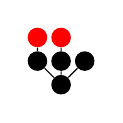
\begin{tikzpicture}[scale=.2]
\node[circle, scale=0.75, fill] (tid0) at (2.25,1.5){};
\node[circle, scale=0.75, fill] (tid1) at (0.75,3){};
\node[circle, scale=0.75, fill, red] (tid4) at (0.75,4.5){};
\draw[](tid1) -- (tid4);
\node[circle, scale=0.75, fill] (tid2) at (2.25,3){};
\node[circle, scale=0.75, fill, red] (tid5) at (2.25,4.5){};
\draw[](tid2) -- (tid5);
\node[circle, scale=0.75, fill] (tid3) at (3.75,3){};
\draw[](tid0) -- (tid1);
\draw[](tid0) -- (tid2);
\draw[](tid0) -- (tid3);
\end{tikzpicture}
\nodepart{two}
\footnotesize{4.125}
\nodepart{three}
\footnotesize{$1$}
};
\node[draw opacity=0, fill opacity=0, anchor=south west] (dummyL) at (-6, -75){};
\node[draw=black, rectangle split, anchor=south west, rectangle split parts=3] (sn0x2620400) at ([xshift=2cm]sn0x261fa80.south east){
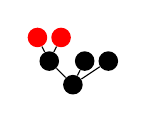
\begin{tikzpicture}[scale=.2]
\node[circle, scale=0.75, fill] (tid0) at (3,1.5){};
\node[circle, scale=0.75, fill] (tid1) at (1.5,3){};
\node[circle, scale=0.75, fill, red] (tid4) at (0.75,4.5){};
\node[circle, scale=0.75, fill, red] (tid5) at (2.25,4.5){};
\draw[](tid1) -- (tid4);
\draw[](tid1) -- (tid5);
\node[circle, scale=0.75, fill] (tid2) at (3.75,3){};
\node[circle, scale=0.75, fill] (tid3) at (5.25,3){};
\draw[](tid0) -- (tid1);
\draw[](tid0) -- (tid2);
\draw[](tid0) -- (tid3);
\end{tikzpicture}
\nodepart{two}
\footnotesize{4.125}
\nodepart{three}
\footnotesize{$1$}
};
\node[draw opacity=0, fill opacity=0, anchor=south west] (dummyL) at (-3, -90){};
\node[draw=black, rectangle split, anchor=south west, rectangle split parts=3] (sn0x261fb40) at ([xshift=2cm]dummyL){
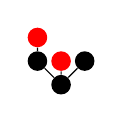
\begin{tikzpicture}[scale=.2]
\node[circle, scale=0.75, fill] (tid0) at (2.25,1.5){};
\node[circle, scale=0.75, fill] (tid1) at (0.75,3){};
\node[circle, scale=0.75, fill, red] (tid4) at (0.75,4.5){};
\draw[](tid1) -- (tid4);
\node[circle, scale=0.75, fill, red] (tid2) at (2.25,3){};
\node[circle, scale=0.75, fill] (tid3) at (3.75,3){};
\draw[](tid0) -- (tid1);
\draw[](tid0) -- (tid2);
\draw[](tid0) -- (tid3);
\end{tikzpicture}
\nodepart{two}
\footnotesize{3.625}
\nodepart{three}
\footnotesize{$50\:50$}
};
\node[draw opacity=0, fill opacity=0, anchor=south west] (dummyL) at (-6, -105){};
\node[draw=black, rectangle split, anchor=south west, rectangle split parts=3] (sn0x261f8e0) at ([xshift=2cm]dummyL){
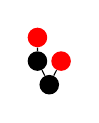
\begin{tikzpicture}[scale=.2]
\node[circle, scale=0.75, fill] (tid0) at (1.5,1.5){};
\node[circle, scale=0.75, fill] (tid1) at (0.75,3){};
\node[circle, scale=0.75, fill, red] (tid3) at (0.75,4.5){};
\draw[](tid1) -- (tid3);
\node[circle, scale=0.75, fill, red] (tid2) at (2.25,3){};
\draw[](tid0) -- (tid1);
\draw[](tid0) -- (tid2);
\end{tikzpicture}
\nodepart{two}
\footnotesize{3.25}
\nodepart{three}
\footnotesize{$50\:50$}
};
\node[draw opacity=0, fill opacity=0, anchor=south west] (dummyL) at (-6, -105){};
\node[draw=black, rectangle split, anchor=south west, rectangle split parts=3] (sn0x261fd90) at ([xshift=2cm]sn0x261f8e0.south east){
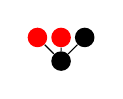
\begin{tikzpicture}[scale=.2]
\node[circle, scale=0.75, fill] (tid0) at (2.25,1.5){};
\node[circle, scale=0.75, fill, red] (tid1) at (0.75,3){};
\node[circle, scale=0.75, fill, red] (tid2) at (2.25,3){};
\node[circle, scale=0.75, fill] (tid3) at (3.75,3){};
\draw[](tid0) -- (tid1);
\draw[](tid0) -- (tid2);
\draw[](tid0) -- (tid3);
\end{tikzpicture}
\nodepart{two}
\footnotesize{3}
\nodepart{three}
\footnotesize{$1$}
};
\node[draw opacity=0, fill opacity=0, anchor=south west] (dummyL) at (-6, -120){};
\node[draw=black, rectangle split, anchor=south west, rectangle split parts=3] (sn0x261fe50) at ([xshift=2cm]dummyL){
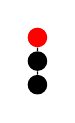
\begin{tikzpicture}[scale=.2]
\node[circle, scale=0.75, fill] (tid0) at (0.75,1.5){};
\node[circle, scale=0.75, fill] (tid1) at (0.75,3){};
\node[circle, scale=0.75, fill, red] (tid2) at (0.75,4.5){};
\draw[](tid1) -- (tid2);
\draw[](tid0) -- (tid1);
\end{tikzpicture}
\nodepart{two}
\footnotesize{3}
\nodepart{three}
\footnotesize{$1$}
};
\node[draw opacity=0, fill opacity=0, anchor=south west] (dummyL) at (-6, -120){};
\node[draw=black, rectangle split, anchor=south west, rectangle split parts=3] (sn0x261ff10) at ([xshift=2cm]sn0x261fe50.south east){

\begin{tikzpicture}[scale=.2]
\node[circle, scale=0.75, fill] (tid0) at (1.5,1.5){};
\node[circle, scale=0.75, fill, red] (tid1) at (0.75,3){};
\node[circle, scale=0.75, fill, red] (tid2) at (2.25,3){};
\draw[](tid0) -- (tid1);
\draw[](tid0) -- (tid2);
\end{tikzpicture}
\nodepart{two}
\footnotesize{2.5}
\nodepart{three}
\footnotesize{$1$}
};
\node[draw opacity=0, fill opacity=0, anchor=south west] (dummyL) at (-3, -135){};
\node[draw=black, rectangle split, anchor=south west, rectangle split parts=3] (sn0x2620120) at ([xshift=2cm]dummyL){

\begin{tikzpicture}[scale=.2]
\node[circle, scale=0.75, fill] (tid0) at (0.75,1.5){};
\node[circle, scale=0.75, fill, red] (tid1) at (0.75,3){};
\draw[](tid0) -- (tid1);
\end{tikzpicture}
\nodepart{two}
\footnotesize{2}
\nodepart{three}
\footnotesize{$1$}
};
\node[draw opacity=0, fill opacity=0, anchor=south west] (dummyL) at (-3, -150){};
\node[draw=black, rectangle split, anchor=south west, rectangle split parts=3] (sn0x26201e0) at ([xshift=2cm]dummyL){

\begin{tikzpicture}[scale=.2]
\node[circle, scale=0.75, fill, red] (tid0) at (0.75,1.5){};
\end{tikzpicture}
\nodepart{two}
\footnotesize{1}
\nodepart{three}
\footnotesize{$$}
};
\draw (sn0x2614278.south) -- (sn0x2611eb0.north);
\draw (sn0x2614278.south) -- (sn0x261e5f0.north);
\draw (sn0x2614278.south) -- (sn0x26163b0.north);
\draw (sn0x2611eb0.south) -- (sn0x2612000.north);
\draw (sn0x2611eb0.south) -- (sn0x26212b0.north);
\draw (sn0x261e5f0.south) -- (sn0x2612000.north);
\draw (sn0x261e5f0.south) -- (sn0x2615a00.north);
\draw (sn0x26163b0.south) -- (sn0x26212b0.north);
\draw (sn0x26163b0.south) -- (sn0x2612000.north);
\draw (sn0x26163b0.south) -- (sn0x2621ec0.north);
\draw (sn0x26163b0.south) -- (sn0x26219b0.north);
\draw (sn0x2612000.south) -- (sn0x2614f90.north);
\draw (sn0x2612000.south) -- (sn0x261e6b0.north);
\draw (sn0x2612000.south) -- (sn0x261f7a0.north);
\draw (sn0x26212b0.south) -- (sn0x261f7a0.north);
\draw (sn0x2615a00.south) -- (sn0x2614f90.north);
\draw (sn0x2621ec0.south) -- (sn0x261f7a0.north);
\draw (sn0x26219b0.south) -- (sn0x261f7a0.north);
\draw (sn0x26219b0.south) -- (sn0x261e6b0.north);
\draw (sn0x2614f90.south) -- (sn0x261fa80.north);
\draw (sn0x261e6b0.south) -- (sn0x261fa80.north);
\draw (sn0x261f7a0.south) -- (sn0x261fa80.north);
\draw (sn0x261f7a0.south) -- (sn0x2620400.north);
\draw (sn0x261fa80.south) -- (sn0x261fb40.north);
\draw (sn0x2620400.south) -- (sn0x261fb40.north);
\draw (sn0x261fb40.south) -- (sn0x261f8e0.north);
\draw (sn0x261fb40.south) -- (sn0x261fd90.north);
\draw (sn0x261f8e0.south) -- (sn0x261fe50.north);
\draw (sn0x261f8e0.south) -- (sn0x261ff10.north);
\draw (sn0x261fd90.south) -- (sn0x261ff10.north);
\draw (sn0x261fe50.south) -- (sn0x2620120.north);
\draw (sn0x261ff10.south) -- (sn0x2620120.north);
\draw (sn0x2620120.south) -- (sn0x26201e0.north);
\end{tikzpicture}

%%% Local Variables:
%%% TeX-master: "thesis/thesis.tex"
%%% End: 
\begin{tikzpicture}[scale=.2, anchor=west]
\node[draw opacity=0, fill opacity=0, anchor=south west] (dummyL) at (-3, -15){};
\node[draw=black, rectangle split, anchor=south west, rectangle split parts=3] (sn0x2614330) at ([xshift=2cm]dummyL){
\begin{tikzpicture}[scale=.2]
\node[circle, scale=0.75, fill] (tid0) at (4.5,1.5){};
\node[circle, scale=0.75, fill] (tid1) at (2.25,3){};
\node[circle, scale=0.75, fill, red] (tid4) at (0.75,4.5){};
\node[circle, scale=0.75, fill] (tid5) at (2.25,4.5){};
\node[circle, scale=0.75, fill] (tid6) at (3.75,4.5){};
\draw[](tid1) -- (tid4);
\draw[](tid1) -- (tid5);
\draw[](tid1) -- (tid6);
\node[circle, scale=0.75, fill] (tid2) at (6,3){};
\node[circle, scale=0.75, fill] (tid7) at (5.25,4.5){};
\node[circle, scale=0.75, fill] (tid8) at (6.75,4.5){};
\draw[](tid2) -- (tid7);
\draw[](tid2) -- (tid8);
\node[circle, scale=0.75, fill] (tid3) at (8.25,3){};
\node[circle, scale=0.75, fill, red] (tid9) at (8.25,4.5){};
\draw[](tid3) -- (tid9);
\draw[](tid0) -- (tid1);
\draw[](tid0) -- (tid2);
\draw[](tid0) -- (tid3);
\end{tikzpicture}
\nodepart{two}
\footnotesize{6.125}
\nodepart{three}
\footnotesize{$50\:25\:25$}
};
\node[draw opacity=0, fill opacity=0, anchor=south west] (dummyL) at (-9, -30){};
\node[draw=black, rectangle split, anchor=south west, rectangle split parts=3] (sn0x26163b0) at ([xshift=2cm]dummyL){
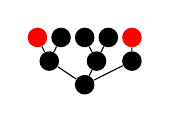
\begin{tikzpicture}[scale=.2]
\node[circle, scale=0.75, fill] (tid0) at (3.75,1.5){};
\node[circle, scale=0.75, fill] (tid1) at (1.5,3){};
\node[circle, scale=0.75, fill, red] (tid4) at (0.75,4.5){};
\node[circle, scale=0.75, fill] (tid5) at (2.25,4.5){};
\draw[](tid1) -- (tid4);
\draw[](tid1) -- (tid5);
\node[circle, scale=0.75, fill] (tid2) at (4.5,3){};
\node[circle, scale=0.75, fill] (tid6) at (3.75,4.5){};
\node[circle, scale=0.75, fill] (tid7) at (5.25,4.5){};
\draw[](tid2) -- (tid6);
\draw[](tid2) -- (tid7);
\node[circle, scale=0.75, fill] (tid3) at (6.75,3){};
\node[circle, scale=0.75, fill, red] (tid8) at (6.75,4.5){};
\draw[](tid3) -- (tid8);
\draw[](tid0) -- (tid1);
\draw[](tid0) -- (tid2);
\draw[](tid0) -- (tid3);
\end{tikzpicture}
\nodepart{two}
\footnotesize{5.625}
\nodepart{three}
\footnotesize{$17\:33\:17\:33$}
};
\node[draw opacity=0, fill opacity=0, anchor=south west] (dummyL) at (-9, -30){};
\node[draw=black, rectangle split, anchor=south west, rectangle split parts=3] (sn0x2623380) at ([xshift=2cm]sn0x26163b0.south east){
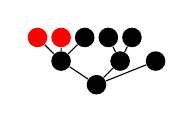
\begin{tikzpicture}[scale=.2]
\node[circle, scale=0.75, fill] (tid0) at (4.5,1.5){};
\node[circle, scale=0.75, fill] (tid1) at (2.25,3){};
\node[circle, scale=0.75, fill, red] (tid4) at (0.75,4.5){};
\node[circle, scale=0.75, fill, red] (tid5) at (2.25,4.5){};
\node[circle, scale=0.75, fill] (tid6) at (3.75,4.5){};
\draw[](tid1) -- (tid4);
\draw[](tid1) -- (tid5);
\draw[](tid1) -- (tid6);
\node[circle, scale=0.75, fill] (tid2) at (6,3){};
\node[circle, scale=0.75, fill] (tid7) at (5.25,4.5){};
\node[circle, scale=0.75, fill] (tid8) at (6.75,4.5){};
\draw[](tid2) -- (tid7);
\draw[](tid2) -- (tid8);
\node[circle, scale=0.75, fill] (tid3) at (8.25,3){};
\draw[](tid0) -- (tid1);
\draw[](tid0) -- (tid2);
\draw[](tid0) -- (tid3);
\end{tikzpicture}
\nodepart{two}
\footnotesize{5.625}
\nodepart{three}
\footnotesize{$33\:67$}
};
\node[draw opacity=0, fill opacity=0, anchor=south west] (dummyL) at (-9, -30){};
\node[draw=black, rectangle split, anchor=south west, rectangle split parts=3] (sn0x2623a70) at ([xshift=2cm]sn0x2623380.south east){
\begin{tikzpicture}[scale=.2]
\node[circle, scale=0.75, fill] (tid0) at (4.5,1.5){};
\node[circle, scale=0.75, fill] (tid1) at (2.25,3){};
\node[circle, scale=0.75, fill, red] (tid4) at (0.75,4.5){};
\node[circle, scale=0.75, fill] (tid5) at (2.25,4.5){};
\node[circle, scale=0.75, fill] (tid6) at (3.75,4.5){};
\draw[](tid1) -- (tid4);
\draw[](tid1) -- (tid5);
\draw[](tid1) -- (tid6);
\node[circle, scale=0.75, fill] (tid2) at (6,3){};
\node[circle, scale=0.75, fill, red] (tid7) at (5.25,4.5){};
\node[circle, scale=0.75, fill] (tid8) at (6.75,4.5){};
\draw[](tid2) -- (tid7);
\draw[](tid2) -- (tid8);
\node[circle, scale=0.75, fill] (tid3) at (8.25,3){};
\draw[](tid0) -- (tid1);
\draw[](tid0) -- (tid2);
\draw[](tid0) -- (tid3);
\end{tikzpicture}
\nodepart{two}
\footnotesize{5.625}
\nodepart{three}
\footnotesize{$17\:33\:33\:17$}
};
\node[draw opacity=0, fill opacity=0, anchor=south west] (dummyL) at (-18, -45){};
\node[draw=black, rectangle split, anchor=south west, rectangle split parts=3] (sn0x26212b0) at ([xshift=2cm]dummyL){
\begin{tikzpicture}[scale=.2]
\node[circle, scale=0.75, fill] (tid0) at (3,1.5){};
\node[circle, scale=0.75, fill] (tid1) at (1.5,3){};
\node[circle, scale=0.75, fill] (tid4) at (0.75,4.5){};
\node[circle, scale=0.75, fill] (tid5) at (2.25,4.5){};
\draw[](tid1) -- (tid4);
\draw[](tid1) -- (tid5);
\node[circle, scale=0.75, fill] (tid2) at (3.75,3){};
\node[circle, scale=0.75, fill, red] (tid6) at (3.75,4.5){};
\draw[](tid2) -- (tid6);
\node[circle, scale=0.75, fill] (tid3) at (5.25,3){};
\node[circle, scale=0.75, fill, red] (tid7) at (5.25,4.5){};
\draw[](tid3) -- (tid7);
\draw[](tid0) -- (tid1);
\draw[](tid0) -- (tid2);
\draw[](tid0) -- (tid3);
\end{tikzpicture}
\nodepart{two}
\footnotesize{5.125}
\nodepart{three}
\footnotesize{$1$}
};
\node[draw opacity=0, fill opacity=0, anchor=south west] (dummyL) at (-18, -45){};
\node[draw=black, rectangle split, anchor=south west, rectangle split parts=3] (sn0x2612000) at ([xshift=2cm]sn0x26212b0.south east){
\begin{tikzpicture}[scale=.2]
\node[circle, scale=0.75, fill] (tid0) at (3,1.5){};
\node[circle, scale=0.75, fill] (tid1) at (1.5,3){};
\node[circle, scale=0.75, fill, red] (tid4) at (0.75,4.5){};
\node[circle, scale=0.75, fill] (tid5) at (2.25,4.5){};
\draw[](tid1) -- (tid4);
\draw[](tid1) -- (tid5);
\node[circle, scale=0.75, fill] (tid2) at (3.75,3){};
\node[circle, scale=0.75, fill, red] (tid6) at (3.75,4.5){};
\draw[](tid2) -- (tid6);
\node[circle, scale=0.75, fill] (tid3) at (5.25,3){};
\node[circle, scale=0.75, fill] (tid7) at (5.25,4.5){};
\draw[](tid3) -- (tid7);
\draw[](tid0) -- (tid1);
\draw[](tid0) -- (tid2);
\draw[](tid0) -- (tid3);
\end{tikzpicture}
\nodepart{two}
\footnotesize{5.125}
\nodepart{three}
\footnotesize{$25\:50\:25$}
};
\node[draw opacity=0, fill opacity=0, anchor=south west] (dummyL) at (-18, -45){};
\node[draw=black, rectangle split, anchor=south west, rectangle split parts=3] (sn0x2621ec0) at ([xshift=2cm]sn0x2612000.south east){
\begin{tikzpicture}[scale=.2]
\node[circle, scale=0.75, fill] (tid0) at (3.75,1.5){};
\node[circle, scale=0.75, fill] (tid1) at (1.5,3){};
\node[circle, scale=0.75, fill, red] (tid4) at (0.75,4.5){};
\node[circle, scale=0.75, fill, red] (tid5) at (2.25,4.5){};
\draw[](tid1) -- (tid4);
\draw[](tid1) -- (tid5);
\node[circle, scale=0.75, fill] (tid2) at (4.5,3){};
\node[circle, scale=0.75, fill] (tid6) at (3.75,4.5){};
\node[circle, scale=0.75, fill] (tid7) at (5.25,4.5){};
\draw[](tid2) -- (tid6);
\draw[](tid2) -- (tid7);
\node[circle, scale=0.75, fill] (tid3) at (6.75,3){};
\draw[](tid0) -- (tid1);
\draw[](tid0) -- (tid2);
\draw[](tid0) -- (tid3);
\end{tikzpicture}
\nodepart{two}
\footnotesize{5.125}
\nodepart{three}
\footnotesize{$1$}
};
\node[draw opacity=0, fill opacity=0, anchor=south west] (dummyL) at (-18, -45){};
\node[draw=black, rectangle split, anchor=south west, rectangle split parts=3] (sn0x26219b0) at ([xshift=2cm]sn0x2621ec0.south east){
\begin{tikzpicture}[scale=.2]
\node[circle, scale=0.75, fill] (tid0) at (3.75,1.5){};
\node[circle, scale=0.75, fill] (tid1) at (1.5,3){};
\node[circle, scale=0.75, fill, red] (tid4) at (0.75,4.5){};
\node[circle, scale=0.75, fill] (tid5) at (2.25,4.5){};
\draw[](tid1) -- (tid4);
\draw[](tid1) -- (tid5);
\node[circle, scale=0.75, fill] (tid2) at (4.5,3){};
\node[circle, scale=0.75, fill, red] (tid6) at (3.75,4.5){};
\node[circle, scale=0.75, fill] (tid7) at (5.25,4.5){};
\draw[](tid2) -- (tid6);
\draw[](tid2) -- (tid7);
\node[circle, scale=0.75, fill] (tid3) at (6.75,3){};
\draw[](tid0) -- (tid1);
\draw[](tid0) -- (tid2);
\draw[](tid0) -- (tid3);
\end{tikzpicture}
\nodepart{two}
\footnotesize{5.125}
\nodepart{three}
\footnotesize{$50\:50$}
};
\node[draw opacity=0, fill opacity=0, anchor=south west] (dummyL) at (-18, -45){};
\node[draw=black, rectangle split, anchor=south west, rectangle split parts=3] (sn0x2622820) at ([xshift=2cm]sn0x26219b0.south east){
\begin{tikzpicture}[scale=.2]
\node[circle, scale=0.75, fill] (tid0) at (3.75,1.5){};
\node[circle, scale=0.75, fill] (tid1) at (2.25,3){};
\node[circle, scale=0.75, fill, red] (tid4) at (0.75,4.5){};
\node[circle, scale=0.75, fill, red] (tid5) at (2.25,4.5){};
\node[circle, scale=0.75, fill] (tid6) at (3.75,4.5){};
\draw[](tid1) -- (tid4);
\draw[](tid1) -- (tid5);
\draw[](tid1) -- (tid6);
\node[circle, scale=0.75, fill] (tid2) at (5.25,3){};
\node[circle, scale=0.75, fill] (tid7) at (5.25,4.5){};
\draw[](tid2) -- (tid7);
\node[circle, scale=0.75, fill] (tid3) at (6.75,3){};
\draw[](tid0) -- (tid1);
\draw[](tid0) -- (tid2);
\draw[](tid0) -- (tid3);
\end{tikzpicture}
\nodepart{two}
\footnotesize{5.125}
\nodepart{three}
\footnotesize{$50\:50$}
};
\node[draw opacity=0, fill opacity=0, anchor=south west] (dummyL) at (-18, -45){};
\node[draw=black, rectangle split, anchor=south west, rectangle split parts=3] (sn0x2622950) at ([xshift=2cm]sn0x2622820.south east){
\begin{tikzpicture}[scale=.2]
\node[circle, scale=0.75, fill] (tid0) at (3.75,1.5){};
\node[circle, scale=0.75, fill] (tid1) at (2.25,3){};
\node[circle, scale=0.75, fill, red] (tid4) at (0.75,4.5){};
\node[circle, scale=0.75, fill] (tid5) at (2.25,4.5){};
\node[circle, scale=0.75, fill] (tid6) at (3.75,4.5){};
\draw[](tid1) -- (tid4);
\draw[](tid1) -- (tid5);
\draw[](tid1) -- (tid6);
\node[circle, scale=0.75, fill] (tid2) at (5.25,3){};
\node[circle, scale=0.75, fill, red] (tid7) at (5.25,4.5){};
\draw[](tid2) -- (tid7);
\node[circle, scale=0.75, fill] (tid3) at (6.75,3){};
\draw[](tid0) -- (tid1);
\draw[](tid0) -- (tid2);
\draw[](tid0) -- (tid3);
\end{tikzpicture}
\nodepart{two}
\footnotesize{5.125}
\nodepart{three}
\footnotesize{$50\:50$}
};
\node[draw opacity=0, fill opacity=0, anchor=south west] (dummyL) at (-12, -60){};
\node[draw=black, rectangle split, anchor=south west, rectangle split parts=3] (sn0x261f7a0) at ([xshift=2cm]dummyL){
\begin{tikzpicture}[scale=.2]
\node[circle, scale=0.75, fill] (tid0) at (3,1.5){};
\node[circle, scale=0.75, fill] (tid1) at (1.5,3){};
\node[circle, scale=0.75, fill, red] (tid4) at (0.75,4.5){};
\node[circle, scale=0.75, fill] (tid5) at (2.25,4.5){};
\draw[](tid1) -- (tid4);
\draw[](tid1) -- (tid5);
\node[circle, scale=0.75, fill] (tid2) at (3.75,3){};
\node[circle, scale=0.75, fill, red] (tid6) at (3.75,4.5){};
\draw[](tid2) -- (tid6);
\node[circle, scale=0.75, fill] (tid3) at (5.25,3){};
\draw[](tid0) -- (tid1);
\draw[](tid0) -- (tid2);
\draw[](tid0) -- (tid3);
\end{tikzpicture}
\nodepart{two}
\footnotesize{4.625}
\nodepart{three}
\footnotesize{$50\:50$}
};
\node[draw opacity=0, fill opacity=0, anchor=south west] (dummyL) at (-12, -60){};
\node[draw=black, rectangle split, anchor=south west, rectangle split parts=3] (sn0x2614f90) at ([xshift=2cm]sn0x261f7a0.south east){
\begin{tikzpicture}[scale=.2]
\node[circle, scale=0.75, fill] (tid0) at (2.25,1.5){};
\node[circle, scale=0.75, fill] (tid1) at (0.75,3){};
\node[circle, scale=0.75, fill, red] (tid4) at (0.75,4.5){};
\draw[](tid1) -- (tid4);
\node[circle, scale=0.75, fill] (tid2) at (2.25,3){};
\node[circle, scale=0.75, fill, red] (tid5) at (2.25,4.5){};
\draw[](tid2) -- (tid5);
\node[circle, scale=0.75, fill] (tid3) at (3.75,3){};
\node[circle, scale=0.75, fill] (tid6) at (3.75,4.5){};
\draw[](tid3) -- (tid6);
\draw[](tid0) -- (tid1);
\draw[](tid0) -- (tid2);
\draw[](tid0) -- (tid3);
\end{tikzpicture}
\nodepart{two}
\footnotesize{4.625}
\nodepart{three}
\footnotesize{$1$}
};
\node[draw opacity=0, fill opacity=0, anchor=south west] (dummyL) at (-12, -60){};
\node[draw=black, rectangle split, anchor=south west, rectangle split parts=3] (sn0x261e6b0) at ([xshift=2cm]sn0x2614f90.south east){
\begin{tikzpicture}[scale=.2]
\node[circle, scale=0.75, fill] (tid0) at (3,1.5){};
\node[circle, scale=0.75, fill] (tid1) at (1.5,3){};
\node[circle, scale=0.75, fill, red] (tid4) at (0.75,4.5){};
\node[circle, scale=0.75, fill, red] (tid5) at (2.25,4.5){};
\draw[](tid1) -- (tid4);
\draw[](tid1) -- (tid5);
\node[circle, scale=0.75, fill] (tid2) at (3.75,3){};
\node[circle, scale=0.75, fill] (tid6) at (3.75,4.5){};
\draw[](tid2) -- (tid6);
\node[circle, scale=0.75, fill] (tid3) at (5.25,3){};
\draw[](tid0) -- (tid1);
\draw[](tid0) -- (tid2);
\draw[](tid0) -- (tid3);
\end{tikzpicture}
\nodepart{two}
\footnotesize{4.625}
\nodepart{three}
\footnotesize{$1$}
};
\node[draw opacity=0, fill opacity=0, anchor=south west] (dummyL) at (-12, -60){};
\node[draw=black, rectangle split, anchor=south west, rectangle split parts=3] (sn0x26232c0) at ([xshift=2cm]sn0x261e6b0.south east){
\begin{tikzpicture}[scale=.2]
\node[circle, scale=0.75, fill] (tid0) at (3.75,1.5){};
\node[circle, scale=0.75, fill] (tid1) at (2.25,3){};
\node[circle, scale=0.75, fill, red] (tid4) at (0.75,4.5){};
\node[circle, scale=0.75, fill, red] (tid5) at (2.25,4.5){};
\node[circle, scale=0.75, fill] (tid6) at (3.75,4.5){};
\draw[](tid1) -- (tid4);
\draw[](tid1) -- (tid5);
\draw[](tid1) -- (tid6);
\node[circle, scale=0.75, fill] (tid2) at (5.25,3){};
\node[circle, scale=0.75, fill] (tid3) at (6.75,3){};
\draw[](tid0) -- (tid1);
\draw[](tid0) -- (tid2);
\draw[](tid0) -- (tid3);
\end{tikzpicture}
\nodepart{two}
\footnotesize{4.625}
\nodepart{three}
\footnotesize{$1$}
};
\node[draw opacity=0, fill opacity=0, anchor=south west] (dummyL) at (-6, -75){};
\node[draw=black, rectangle split, anchor=south west, rectangle split parts=3] (sn0x261fa80) at ([xshift=2cm]dummyL){
\begin{tikzpicture}[scale=.2]
\node[circle, scale=0.75, fill] (tid0) at (2.25,1.5){};
\node[circle, scale=0.75, fill] (tid1) at (0.75,3){};
\node[circle, scale=0.75, fill, red] (tid4) at (0.75,4.5){};
\draw[](tid1) -- (tid4);
\node[circle, scale=0.75, fill] (tid2) at (2.25,3){};
\node[circle, scale=0.75, fill, red] (tid5) at (2.25,4.5){};
\draw[](tid2) -- (tid5);
\node[circle, scale=0.75, fill] (tid3) at (3.75,3){};
\draw[](tid0) -- (tid1);
\draw[](tid0) -- (tid2);
\draw[](tid0) -- (tid3);
\end{tikzpicture}
\nodepart{two}
\footnotesize{4.125}
\nodepart{three}
\footnotesize{$1$}
};
\node[draw opacity=0, fill opacity=0, anchor=south west] (dummyL) at (-6, -75){};
\node[draw=black, rectangle split, anchor=south west, rectangle split parts=3] (sn0x2620400) at ([xshift=2cm]sn0x261fa80.south east){
\begin{tikzpicture}[scale=.2]
\node[circle, scale=0.75, fill] (tid0) at (3,1.5){};
\node[circle, scale=0.75, fill] (tid1) at (1.5,3){};
\node[circle, scale=0.75, fill, red] (tid4) at (0.75,4.5){};
\node[circle, scale=0.75, fill, red] (tid5) at (2.25,4.5){};
\draw[](tid1) -- (tid4);
\draw[](tid1) -- (tid5);
\node[circle, scale=0.75, fill] (tid2) at (3.75,3){};
\node[circle, scale=0.75, fill] (tid3) at (5.25,3){};
\draw[](tid0) -- (tid1);
\draw[](tid0) -- (tid2);
\draw[](tid0) -- (tid3);
\end{tikzpicture}
\nodepart{two}
\footnotesize{4.125}
\nodepart{three}
\footnotesize{$1$}
};
\node[draw opacity=0, fill opacity=0, anchor=south west] (dummyL) at (-3, -90){};
\node[draw=black, rectangle split, anchor=south west, rectangle split parts=3] (sn0x261fb40) at ([xshift=2cm]dummyL){
\begin{tikzpicture}[scale=.2]
\node[circle, scale=0.75, fill] (tid0) at (2.25,1.5){};
\node[circle, scale=0.75, fill] (tid1) at (0.75,3){};
\node[circle, scale=0.75, fill, red] (tid4) at (0.75,4.5){};
\draw[](tid1) -- (tid4);
\node[circle, scale=0.75, fill, red] (tid2) at (2.25,3){};
\node[circle, scale=0.75, fill] (tid3) at (3.75,3){};
\draw[](tid0) -- (tid1);
\draw[](tid0) -- (tid2);
\draw[](tid0) -- (tid3);
\end{tikzpicture}
\nodepart{two}
\footnotesize{3.625}
\nodepart{three}
\footnotesize{$50\:50$}
};
\node[draw opacity=0, fill opacity=0, anchor=south west] (dummyL) at (-6, -105){};
\node[draw=black, rectangle split, anchor=south west, rectangle split parts=3] (sn0x261f8e0) at ([xshift=2cm]dummyL){
\begin{tikzpicture}[scale=.2]
\node[circle, scale=0.75, fill] (tid0) at (1.5,1.5){};
\node[circle, scale=0.75, fill] (tid1) at (0.75,3){};
\node[circle, scale=0.75, fill, red] (tid3) at (0.75,4.5){};
\draw[](tid1) -- (tid3);
\node[circle, scale=0.75, fill, red] (tid2) at (2.25,3){};
\draw[](tid0) -- (tid1);
\draw[](tid0) -- (tid2);
\end{tikzpicture}
\nodepart{two}
\footnotesize{3.25}
\nodepart{three}
\footnotesize{$50\:50$}
};
\node[draw opacity=0, fill opacity=0, anchor=south west] (dummyL) at (-6, -105){};
\node[draw=black, rectangle split, anchor=south west, rectangle split parts=3] (sn0x261fd90) at ([xshift=2cm]sn0x261f8e0.south east){
\begin{tikzpicture}[scale=.2]
\node[circle, scale=0.75, fill] (tid0) at (2.25,1.5){};
\node[circle, scale=0.75, fill, red] (tid1) at (0.75,3){};
\node[circle, scale=0.75, fill, red] (tid2) at (2.25,3){};
\node[circle, scale=0.75, fill] (tid3) at (3.75,3){};
\draw[](tid0) -- (tid1);
\draw[](tid0) -- (tid2);
\draw[](tid0) -- (tid3);
\end{tikzpicture}
\nodepart{two}
\footnotesize{3}
\nodepart{three}
\footnotesize{$1$}
};
\node[draw opacity=0, fill opacity=0, anchor=south west] (dummyL) at (-6, -120){};
\node[draw=black, rectangle split, anchor=south west, rectangle split parts=3] (sn0x261fe50) at ([xshift=2cm]dummyL){
\begin{tikzpicture}[scale=.2]
\node[circle, scale=0.75, fill] (tid0) at (0.75,1.5){};
\node[circle, scale=0.75, fill] (tid1) at (0.75,3){};
\node[circle, scale=0.75, fill, red] (tid2) at (0.75,4.5){};
\draw[](tid1) -- (tid2);
\draw[](tid0) -- (tid1);
\end{tikzpicture}
\nodepart{two}
\footnotesize{3}
\nodepart{three}
\footnotesize{$1$}
};
\node[draw opacity=0, fill opacity=0, anchor=south west] (dummyL) at (-6, -120){};
\node[draw=black, rectangle split, anchor=south west, rectangle split parts=3] (sn0x261ff10) at ([xshift=2cm]sn0x261fe50.south east){
\begin{tikzpicture}[scale=.2]
\node[circle, scale=0.75, fill] (tid0) at (1.5,1.5){};
\node[circle, scale=0.75, fill, red] (tid1) at (0.75,3){};
\node[circle, scale=0.75, fill, red] (tid2) at (2.25,3){};
\draw[](tid0) -- (tid1);
\draw[](tid0) -- (tid2);
\end{tikzpicture}
\nodepart{two}
\footnotesize{2.5}
\nodepart{three}
\footnotesize{$1$}
};
\node[draw opacity=0, fill opacity=0, anchor=south west] (dummyL) at (-3, -135){};
\node[draw=black, rectangle split, anchor=south west, rectangle split parts=3] (sn0x2620120) at ([xshift=2cm]dummyL){
\begin{tikzpicture}[scale=.2]
\node[circle, scale=0.75, fill] (tid0) at (0.75,1.5){};
\node[circle, scale=0.75, fill, red] (tid1) at (0.75,3){};
\draw[](tid0) -- (tid1);
\end{tikzpicture}
\nodepart{two}
\footnotesize{2}
\nodepart{three}
\footnotesize{$1$}
};
\node[draw opacity=0, fill opacity=0, anchor=south west] (dummyL) at (-3, -150){};
\node[draw=black, rectangle split, anchor=south west, rectangle split parts=3] (sn0x26201e0) at ([xshift=2cm]dummyL){
\begin{tikzpicture}[scale=.2]
\node[circle, scale=0.75, fill, red] (tid0) at (0.75,1.5){};
\end{tikzpicture}
\nodepart{two}
\footnotesize{1}
\nodepart{three}
\footnotesize{$$}
};
\draw (sn0x2614330.south) -- (sn0x26163b0.north);
\draw (sn0x2614330.south) -- (sn0x2623380.north);
\draw (sn0x2614330.south) -- (sn0x2623a70.north);
\draw (sn0x26163b0.south) -- (sn0x26212b0.north);
\draw (sn0x26163b0.south) -- (sn0x2612000.north);
\draw (sn0x26163b0.south) -- (sn0x2621ec0.north);
\draw (sn0x26163b0.south) -- (sn0x26219b0.north);
\draw (sn0x2623380.south) -- (sn0x2621ec0.north);
\draw (sn0x2623380.south) -- (sn0x26219b0.north);
\draw (sn0x2623a70.south) -- (sn0x26219b0.north);
\draw (sn0x2623a70.south) -- (sn0x2621ec0.north);
\draw (sn0x2623a70.south) -- (sn0x2622820.north);
\draw (sn0x2623a70.south) -- (sn0x2622950.north);
\draw (sn0x26212b0.south) -- (sn0x261f7a0.north);
\draw (sn0x2612000.south) -- (sn0x2614f90.north);
\draw (sn0x2612000.south) -- (sn0x261e6b0.north);
\draw (sn0x2612000.south) -- (sn0x261f7a0.north);
\draw (sn0x2621ec0.south) -- (sn0x261f7a0.north);
\draw (sn0x26219b0.south) -- (sn0x261f7a0.north);
\draw (sn0x26219b0.south) -- (sn0x261e6b0.north);
\draw (sn0x2622820.south) -- (sn0x261e6b0.north);
\draw (sn0x2622820.south) -- (sn0x261f7a0.north);
\draw (sn0x2622950.south) -- (sn0x261f7a0.north);
\draw (sn0x2622950.south) -- (sn0x26232c0.north);
\draw (sn0x261f7a0.south) -- (sn0x261fa80.north);
\draw (sn0x261f7a0.south) -- (sn0x2620400.north);
\draw (sn0x2614f90.south) -- (sn0x261fa80.north);
\draw (sn0x261e6b0.south) -- (sn0x261fa80.north);
\draw (sn0x26232c0.south) -- (sn0x2620400.north);
\draw (sn0x261fa80.south) -- (sn0x261fb40.north);
\draw (sn0x2620400.south) -- (sn0x261fb40.north);
\draw (sn0x261fb40.south) -- (sn0x261f8e0.north);
\draw (sn0x261fb40.south) -- (sn0x261fd90.north);
\draw (sn0x261f8e0.south) -- (sn0x261fe50.north);
\draw (sn0x261f8e0.south) -- (sn0x261ff10.north);
\draw (sn0x261fd90.south) -- (sn0x261ff10.north);
\draw (sn0x261fe50.south) -- (sn0x2620120.north);
\draw (sn0x261ff10.south) -- (sn0x2620120.north);
\draw (sn0x2620120.south) -- (sn0x26201e0.north);
\end{tikzpicture}

%%% Local Variables:
%%% TeX-master: "thesis/thesis.tex"
%%% End: 
\begin{tikzpicture}[scale=.2, anchor=west]
\node[draw opacity=0, fill opacity=0, anchor=south west] (dummyL) at (-3, -15){};
\node[draw=black, rectangle split, anchor=south west, rectangle split parts=3] (sn0x26143e8) at ([xshift=2cm]dummyL){
\begin{tikzpicture}[scale=.2]
\node[circle, scale=0.75, fill] (tid0) at (4.5,1.5){};
\node[circle, scale=0.75, fill] (tid1) at (2.25,3){};
\node[circle, scale=0.75, fill] (tid4) at (0.75,4.5){};
\node[circle, scale=0.75, fill] (tid5) at (2.25,4.5){};
\node[circle, scale=0.75, fill] (tid6) at (3.75,4.5){};
\draw[](tid1) -- (tid4);
\draw[](tid1) -- (tid5);
\draw[](tid1) -- (tid6);
\node[circle, scale=0.75, fill] (tid2) at (6,3){};
\node[circle, scale=0.75, fill, red] (tid7) at (5.25,4.5){};
\node[circle, scale=0.75, fill, red] (tid8) at (6.75,4.5){};
\draw[](tid2) -- (tid7);
\draw[](tid2) -- (tid8);
\node[circle, scale=0.75, fill] (tid3) at (8.25,3){};
\node[circle, scale=0.75, fill] (tid9) at (8.25,4.5){};
\draw[](tid3) -- (tid9);
\draw[](tid0) -- (tid1);
\draw[](tid0) -- (tid2);
\draw[](tid0) -- (tid3);
\end{tikzpicture}
\nodepart{two}
\footnotesize{6.125}
\nodepart{three}
\footnotesize{$75\:25$}
};
\node[draw opacity=0, fill opacity=0, anchor=south west] (dummyL) at (-6, -30){};
\node[draw=black, rectangle split, anchor=south west, rectangle split parts=3] (sn0x26126f0) at ([xshift=2cm]dummyL){
\begin{tikzpicture}[scale=.2]
\node[circle, scale=0.75, fill] (tid0) at (3.75,1.5){};
\node[circle, scale=0.75, fill] (tid1) at (2.25,3){};
\node[circle, scale=0.75, fill, red] (tid4) at (0.75,4.5){};
\node[circle, scale=0.75, fill] (tid5) at (2.25,4.5){};
\node[circle, scale=0.75, fill] (tid6) at (3.75,4.5){};
\draw[](tid1) -- (tid4);
\draw[](tid1) -- (tid5);
\draw[](tid1) -- (tid6);
\node[circle, scale=0.75, fill] (tid2) at (5.25,3){};
\node[circle, scale=0.75, fill, red] (tid7) at (5.25,4.5){};
\draw[](tid2) -- (tid7);
\node[circle, scale=0.75, fill] (tid3) at (6.75,3){};
\node[circle, scale=0.75, fill] (tid8) at (6.75,4.5){};
\draw[](tid3) -- (tid8);
\draw[](tid0) -- (tid1);
\draw[](tid0) -- (tid2);
\draw[](tid0) -- (tid3);
\end{tikzpicture}
\nodepart{two}
\footnotesize{5.625}
\nodepart{three}
\footnotesize{$33\:17\:33\:17$}
};
\node[draw opacity=0, fill opacity=0, anchor=south west] (dummyL) at (-6, -30){};
\node[draw=black, rectangle split, anchor=south west, rectangle split parts=3] (sn0x2623fc0) at ([xshift=2cm]sn0x26126f0.south east){
\begin{tikzpicture}[scale=.2]
\node[circle, scale=0.75, fill] (tid0) at (3.75,1.5){};
\node[circle, scale=0.75, fill] (tid1) at (2.25,3){};
\node[circle, scale=0.75, fill] (tid4) at (0.75,4.5){};
\node[circle, scale=0.75, fill] (tid5) at (2.25,4.5){};
\node[circle, scale=0.75, fill] (tid6) at (3.75,4.5){};
\draw[](tid1) -- (tid4);
\draw[](tid1) -- (tid5);
\draw[](tid1) -- (tid6);
\node[circle, scale=0.75, fill] (tid2) at (5.25,3){};
\node[circle, scale=0.75, fill, red] (tid7) at (5.25,4.5){};
\draw[](tid2) -- (tid7);
\node[circle, scale=0.75, fill] (tid3) at (6.75,3){};
\node[circle, scale=0.75, fill, red] (tid8) at (6.75,4.5){};
\draw[](tid3) -- (tid8);
\draw[](tid0) -- (tid1);
\draw[](tid0) -- (tid2);
\draw[](tid0) -- (tid3);
\end{tikzpicture}
\nodepart{two}
\footnotesize{5.625}
\nodepart{three}
\footnotesize{$1$}
};
\node[draw opacity=0, fill opacity=0, anchor=south west] (dummyL) at (-12, -45){};
\node[draw=black, rectangle split, anchor=south west, rectangle split parts=3] (sn0x2612000) at ([xshift=2cm]dummyL){
\begin{tikzpicture}[scale=.2]
\node[circle, scale=0.75, fill] (tid0) at (3,1.5){};
\node[circle, scale=0.75, fill] (tid1) at (1.5,3){};
\node[circle, scale=0.75, fill, red] (tid4) at (0.75,4.5){};
\node[circle, scale=0.75, fill] (tid5) at (2.25,4.5){};
\draw[](tid1) -- (tid4);
\draw[](tid1) -- (tid5);
\node[circle, scale=0.75, fill] (tid2) at (3.75,3){};
\node[circle, scale=0.75, fill, red] (tid6) at (3.75,4.5){};
\draw[](tid2) -- (tid6);
\node[circle, scale=0.75, fill] (tid3) at (5.25,3){};
\node[circle, scale=0.75, fill] (tid7) at (5.25,4.5){};
\draw[](tid3) -- (tid7);
\draw[](tid0) -- (tid1);
\draw[](tid0) -- (tid2);
\draw[](tid0) -- (tid3);
\end{tikzpicture}
\nodepart{two}
\footnotesize{5.125}
\nodepart{three}
\footnotesize{$50\:25\:25$}
};
\node[draw opacity=0, fill opacity=0, anchor=south west] (dummyL) at (-12, -45){};
\node[draw=black, rectangle split, anchor=south west, rectangle split parts=3] (sn0x26212b0) at ([xshift=2cm]sn0x2612000.south east){
\begin{tikzpicture}[scale=.2]
\node[circle, scale=0.75, fill] (tid0) at (3,1.5){};
\node[circle, scale=0.75, fill] (tid1) at (1.5,3){};
\node[circle, scale=0.75, fill] (tid4) at (0.75,4.5){};
\node[circle, scale=0.75, fill] (tid5) at (2.25,4.5){};
\draw[](tid1) -- (tid4);
\draw[](tid1) -- (tid5);
\node[circle, scale=0.75, fill] (tid2) at (3.75,3){};
\node[circle, scale=0.75, fill, red] (tid6) at (3.75,4.5){};
\draw[](tid2) -- (tid6);
\node[circle, scale=0.75, fill] (tid3) at (5.25,3){};
\node[circle, scale=0.75, fill, red] (tid7) at (5.25,4.5){};
\draw[](tid3) -- (tid7);
\draw[](tid0) -- (tid1);
\draw[](tid0) -- (tid2);
\draw[](tid0) -- (tid3);
\end{tikzpicture}
\nodepart{two}
\footnotesize{5.125}
\nodepart{three}
\footnotesize{$1$}
};
\node[draw opacity=0, fill opacity=0, anchor=south west] (dummyL) at (-12, -45){};
\node[draw=black, rectangle split, anchor=south west, rectangle split parts=3] (sn0x2622820) at ([xshift=2cm]sn0x26212b0.south east){
\begin{tikzpicture}[scale=.2]
\node[circle, scale=0.75, fill] (tid0) at (3.75,1.5){};
\node[circle, scale=0.75, fill] (tid1) at (2.25,3){};
\node[circle, scale=0.75, fill, red] (tid4) at (0.75,4.5){};
\node[circle, scale=0.75, fill, red] (tid5) at (2.25,4.5){};
\node[circle, scale=0.75, fill] (tid6) at (3.75,4.5){};
\draw[](tid1) -- (tid4);
\draw[](tid1) -- (tid5);
\draw[](tid1) -- (tid6);
\node[circle, scale=0.75, fill] (tid2) at (5.25,3){};
\node[circle, scale=0.75, fill] (tid7) at (5.25,4.5){};
\draw[](tid2) -- (tid7);
\node[circle, scale=0.75, fill] (tid3) at (6.75,3){};
\draw[](tid0) -- (tid1);
\draw[](tid0) -- (tid2);
\draw[](tid0) -- (tid3);
\end{tikzpicture}
\nodepart{two}
\footnotesize{5.125}
\nodepart{three}
\footnotesize{$50\:50$}
};
\node[draw opacity=0, fill opacity=0, anchor=south west] (dummyL) at (-12, -45){};
\node[draw=black, rectangle split, anchor=south west, rectangle split parts=3] (sn0x2622950) at ([xshift=2cm]sn0x2622820.south east){
\begin{tikzpicture}[scale=.2]
\node[circle, scale=0.75, fill] (tid0) at (3.75,1.5){};
\node[circle, scale=0.75, fill] (tid1) at (2.25,3){};
\node[circle, scale=0.75, fill, red] (tid4) at (0.75,4.5){};
\node[circle, scale=0.75, fill] (tid5) at (2.25,4.5){};
\node[circle, scale=0.75, fill] (tid6) at (3.75,4.5){};
\draw[](tid1) -- (tid4);
\draw[](tid1) -- (tid5);
\draw[](tid1) -- (tid6);
\node[circle, scale=0.75, fill] (tid2) at (5.25,3){};
\node[circle, scale=0.75, fill, red] (tid7) at (5.25,4.5){};
\draw[](tid2) -- (tid7);
\node[circle, scale=0.75, fill] (tid3) at (6.75,3){};
\draw[](tid0) -- (tid1);
\draw[](tid0) -- (tid2);
\draw[](tid0) -- (tid3);
\end{tikzpicture}
\nodepart{two}
\footnotesize{5.125}
\nodepart{three}
\footnotesize{$50\:50$}
};
\node[draw opacity=0, fill opacity=0, anchor=south west] (dummyL) at (-12, -60){};
\node[draw=black, rectangle split, anchor=south west, rectangle split parts=3] (sn0x2614f90) at ([xshift=2cm]dummyL){
\begin{tikzpicture}[scale=.2]
\node[circle, scale=0.75, fill] (tid0) at (2.25,1.5){};
\node[circle, scale=0.75, fill] (tid1) at (0.75,3){};
\node[circle, scale=0.75, fill, red] (tid4) at (0.75,4.5){};
\draw[](tid1) -- (tid4);
\node[circle, scale=0.75, fill] (tid2) at (2.25,3){};
\node[circle, scale=0.75, fill, red] (tid5) at (2.25,4.5){};
\draw[](tid2) -- (tid5);
\node[circle, scale=0.75, fill] (tid3) at (3.75,3){};
\node[circle, scale=0.75, fill] (tid6) at (3.75,4.5){};
\draw[](tid3) -- (tid6);
\draw[](tid0) -- (tid1);
\draw[](tid0) -- (tid2);
\draw[](tid0) -- (tid3);
\end{tikzpicture}
\nodepart{two}
\footnotesize{4.625}
\nodepart{three}
\footnotesize{$1$}
};
\node[draw opacity=0, fill opacity=0, anchor=south west] (dummyL) at (-12, -60){};
\node[draw=black, rectangle split, anchor=south west, rectangle split parts=3] (sn0x261e6b0) at ([xshift=2cm]sn0x2614f90.south east){
\begin{tikzpicture}[scale=.2]
\node[circle, scale=0.75, fill] (tid0) at (3,1.5){};
\node[circle, scale=0.75, fill] (tid1) at (1.5,3){};
\node[circle, scale=0.75, fill, red] (tid4) at (0.75,4.5){};
\node[circle, scale=0.75, fill, red] (tid5) at (2.25,4.5){};
\draw[](tid1) -- (tid4);
\draw[](tid1) -- (tid5);
\node[circle, scale=0.75, fill] (tid2) at (3.75,3){};
\node[circle, scale=0.75, fill] (tid6) at (3.75,4.5){};
\draw[](tid2) -- (tid6);
\node[circle, scale=0.75, fill] (tid3) at (5.25,3){};
\draw[](tid0) -- (tid1);
\draw[](tid0) -- (tid2);
\draw[](tid0) -- (tid3);
\end{tikzpicture}
\nodepart{two}
\footnotesize{4.625}
\nodepart{three}
\footnotesize{$1$}
};
\node[draw opacity=0, fill opacity=0, anchor=south west] (dummyL) at (-12, -60){};
\node[draw=black, rectangle split, anchor=south west, rectangle split parts=3] (sn0x261f7a0) at ([xshift=2cm]sn0x261e6b0.south east){
\begin{tikzpicture}[scale=.2]
\node[circle, scale=0.75, fill] (tid0) at (3,1.5){};
\node[circle, scale=0.75, fill] (tid1) at (1.5,3){};
\node[circle, scale=0.75, fill, red] (tid4) at (0.75,4.5){};
\node[circle, scale=0.75, fill] (tid5) at (2.25,4.5){};
\draw[](tid1) -- (tid4);
\draw[](tid1) -- (tid5);
\node[circle, scale=0.75, fill] (tid2) at (3.75,3){};
\node[circle, scale=0.75, fill, red] (tid6) at (3.75,4.5){};
\draw[](tid2) -- (tid6);
\node[circle, scale=0.75, fill] (tid3) at (5.25,3){};
\draw[](tid0) -- (tid1);
\draw[](tid0) -- (tid2);
\draw[](tid0) -- (tid3);
\end{tikzpicture}
\nodepart{two}
\footnotesize{4.625}
\nodepart{three}
\footnotesize{$50\:50$}
};
\node[draw opacity=0, fill opacity=0, anchor=south west] (dummyL) at (-12, -60){};
\node[draw=black, rectangle split, anchor=south west, rectangle split parts=3] (sn0x26232c0) at ([xshift=2cm]sn0x261f7a0.south east){
\begin{tikzpicture}[scale=.2]
\node[circle, scale=0.75, fill] (tid0) at (3.75,1.5){};
\node[circle, scale=0.75, fill] (tid1) at (2.25,3){};
\node[circle, scale=0.75, fill, red] (tid4) at (0.75,4.5){};
\node[circle, scale=0.75, fill, red] (tid5) at (2.25,4.5){};
\node[circle, scale=0.75, fill] (tid6) at (3.75,4.5){};
\draw[](tid1) -- (tid4);
\draw[](tid1) -- (tid5);
\draw[](tid1) -- (tid6);
\node[circle, scale=0.75, fill] (tid2) at (5.25,3){};
\node[circle, scale=0.75, fill] (tid3) at (6.75,3){};
\draw[](tid0) -- (tid1);
\draw[](tid0) -- (tid2);
\draw[](tid0) -- (tid3);
\end{tikzpicture}
\nodepart{two}
\footnotesize{4.625}
\nodepart{three}
\footnotesize{$1$}
};
\node[draw opacity=0, fill opacity=0, anchor=south west] (dummyL) at (-6, -75){};
\node[draw=black, rectangle split, anchor=south west, rectangle split parts=3] (sn0x261fa80) at ([xshift=2cm]dummyL){
\begin{tikzpicture}[scale=.2]
\node[circle, scale=0.75, fill] (tid0) at (2.25,1.5){};
\node[circle, scale=0.75, fill] (tid1) at (0.75,3){};
\node[circle, scale=0.75, fill, red] (tid4) at (0.75,4.5){};
\draw[](tid1) -- (tid4);
\node[circle, scale=0.75, fill] (tid2) at (2.25,3){};
\node[circle, scale=0.75, fill, red] (tid5) at (2.25,4.5){};
\draw[](tid2) -- (tid5);
\node[circle, scale=0.75, fill] (tid3) at (3.75,3){};
\draw[](tid0) -- (tid1);
\draw[](tid0) -- (tid2);
\draw[](tid0) -- (tid3);
\end{tikzpicture}
\nodepart{two}
\footnotesize{4.125}
\nodepart{three}
\footnotesize{$1$}
};
\node[draw opacity=0, fill opacity=0, anchor=south west] (dummyL) at (-6, -75){};
\node[draw=black, rectangle split, anchor=south west, rectangle split parts=3] (sn0x2620400) at ([xshift=2cm]sn0x261fa80.south east){
\begin{tikzpicture}[scale=.2]
\node[circle, scale=0.75, fill] (tid0) at (3,1.5){};
\node[circle, scale=0.75, fill] (tid1) at (1.5,3){};
\node[circle, scale=0.75, fill, red] (tid4) at (0.75,4.5){};
\node[circle, scale=0.75, fill, red] (tid5) at (2.25,4.5){};
\draw[](tid1) -- (tid4);
\draw[](tid1) -- (tid5);
\node[circle, scale=0.75, fill] (tid2) at (3.75,3){};
\node[circle, scale=0.75, fill] (tid3) at (5.25,3){};
\draw[](tid0) -- (tid1);
\draw[](tid0) -- (tid2);
\draw[](tid0) -- (tid3);
\end{tikzpicture}
\nodepart{two}
\footnotesize{4.125}
\nodepart{three}
\footnotesize{$1$}
};
\node[draw opacity=0, fill opacity=0, anchor=south west] (dummyL) at (-3, -90){};
\node[draw=black, rectangle split, anchor=south west, rectangle split parts=3] (sn0x261fb40) at ([xshift=2cm]dummyL){
\begin{tikzpicture}[scale=.2]
\node[circle, scale=0.75, fill] (tid0) at (2.25,1.5){};
\node[circle, scale=0.75, fill] (tid1) at (0.75,3){};
\node[circle, scale=0.75, fill, red] (tid4) at (0.75,4.5){};
\draw[](tid1) -- (tid4);
\node[circle, scale=0.75, fill, red] (tid2) at (2.25,3){};
\node[circle, scale=0.75, fill] (tid3) at (3.75,3){};
\draw[](tid0) -- (tid1);
\draw[](tid0) -- (tid2);
\draw[](tid0) -- (tid3);
\end{tikzpicture}
\nodepart{two}
\footnotesize{3.625}
\nodepart{three}
\footnotesize{$50\:50$}
};
\node[draw opacity=0, fill opacity=0, anchor=south west] (dummyL) at (-6, -105){};
\node[draw=black, rectangle split, anchor=south west, rectangle split parts=3] (sn0x261f8e0) at ([xshift=2cm]dummyL){
\begin{tikzpicture}[scale=.2]
\node[circle, scale=0.75, fill] (tid0) at (1.5,1.5){};
\node[circle, scale=0.75, fill] (tid1) at (0.75,3){};
\node[circle, scale=0.75, fill, red] (tid3) at (0.75,4.5){};
\draw[](tid1) -- (tid3);
\node[circle, scale=0.75, fill, red] (tid2) at (2.25,3){};
\draw[](tid0) -- (tid1);
\draw[](tid0) -- (tid2);
\end{tikzpicture}
\nodepart{two}
\footnotesize{3.25}
\nodepart{three}
\footnotesize{$50\:50$}
};
\node[draw opacity=0, fill opacity=0, anchor=south west] (dummyL) at (-6, -105){};
\node[draw=black, rectangle split, anchor=south west, rectangle split parts=3] (sn0x261fd90) at ([xshift=2cm]sn0x261f8e0.south east){
\begin{tikzpicture}[scale=.2]
\node[circle, scale=0.75, fill] (tid0) at (2.25,1.5){};
\node[circle, scale=0.75, fill, red] (tid1) at (0.75,3){};
\node[circle, scale=0.75, fill, red] (tid2) at (2.25,3){};
\node[circle, scale=0.75, fill] (tid3) at (3.75,3){};
\draw[](tid0) -- (tid1);
\draw[](tid0) -- (tid2);
\draw[](tid0) -- (tid3);
\end{tikzpicture}
\nodepart{two}
\footnotesize{3}
\nodepart{three}
\footnotesize{$1$}
};
\node[draw opacity=0, fill opacity=0, anchor=south west] (dummyL) at (-6, -120){};
\node[draw=black, rectangle split, anchor=south west, rectangle split parts=3] (sn0x261fe50) at ([xshift=2cm]dummyL){
\begin{tikzpicture}[scale=.2]
\node[circle, scale=0.75, fill] (tid0) at (0.75,1.5){};
\node[circle, scale=0.75, fill] (tid1) at (0.75,3){};
\node[circle, scale=0.75, fill, red] (tid2) at (0.75,4.5){};
\draw[](tid1) -- (tid2);
\draw[](tid0) -- (tid1);
\end{tikzpicture}
\nodepart{two}
\footnotesize{3}
\nodepart{three}
\footnotesize{$1$}
};
\node[draw opacity=0, fill opacity=0, anchor=south west] (dummyL) at (-6, -120){};
\node[draw=black, rectangle split, anchor=south west, rectangle split parts=3] (sn0x261ff10) at ([xshift=2cm]sn0x261fe50.south east){
\begin{tikzpicture}[scale=.2]
\node[circle, scale=0.75, fill] (tid0) at (1.5,1.5){};
\node[circle, scale=0.75, fill, red] (tid1) at (0.75,3){};
\node[circle, scale=0.75, fill, red] (tid2) at (2.25,3){};
\draw[](tid0) -- (tid1);
\draw[](tid0) -- (tid2);
\end{tikzpicture}
\nodepart{two}
\footnotesize{2.5}
\nodepart{three}
\footnotesize{$1$}
};
\node[draw opacity=0, fill opacity=0, anchor=south west] (dummyL) at (-3, -135){};
\node[draw=black, rectangle split, anchor=south west, rectangle split parts=3] (sn0x2620120) at ([xshift=2cm]dummyL){
\begin{tikzpicture}[scale=.2]
\node[circle, scale=0.75, fill] (tid0) at (0.75,1.5){};
\node[circle, scale=0.75, fill, red] (tid1) at (0.75,3){};
\draw[](tid0) -- (tid1);
\end{tikzpicture}
\nodepart{two}
\footnotesize{2}
\nodepart{three}
\footnotesize{$1$}
};
\node[draw opacity=0, fill opacity=0, anchor=south west] (dummyL) at (-3, -150){};
\node[draw=black, rectangle split, anchor=south west, rectangle split parts=3] (sn0x26201e0) at ([xshift=2cm]dummyL){
\begin{tikzpicture}[scale=.2]
\node[circle, scale=0.75, fill, red] (tid0) at (0.75,1.5){};
\end{tikzpicture}
\nodepart{two}
\footnotesize{1}
\nodepart{three}
\footnotesize{$$}
};
\draw (sn0x26143e8.south) -- (sn0x26126f0.north);
\draw (sn0x26143e8.south) -- (sn0x2623fc0.north);
\draw (sn0x26126f0.south) -- (sn0x2612000.north);
\draw (sn0x26126f0.south) -- (sn0x26212b0.north);
\draw (sn0x26126f0.south) -- (sn0x2622820.north);
\draw (sn0x26126f0.south) -- (sn0x2622950.north);
\draw (sn0x2623fc0.south) -- (sn0x2622950.north);
\draw (sn0x2612000.south) -- (sn0x2614f90.north);
\draw (sn0x2612000.south) -- (sn0x261e6b0.north);
\draw (sn0x2612000.south) -- (sn0x261f7a0.north);
\draw (sn0x26212b0.south) -- (sn0x261f7a0.north);
\draw (sn0x2622820.south) -- (sn0x261e6b0.north);
\draw (sn0x2622820.south) -- (sn0x261f7a0.north);
\draw (sn0x2622950.south) -- (sn0x261f7a0.north);
\draw (sn0x2622950.south) -- (sn0x26232c0.north);
\draw (sn0x2614f90.south) -- (sn0x261fa80.north);
\draw (sn0x261e6b0.south) -- (sn0x261fa80.north);
\draw (sn0x261f7a0.south) -- (sn0x261fa80.north);
\draw (sn0x261f7a0.south) -- (sn0x2620400.north);
\draw (sn0x26232c0.south) -- (sn0x2620400.north);
\draw (sn0x261fa80.south) -- (sn0x261fb40.north);
\draw (sn0x2620400.south) -- (sn0x261fb40.north);
\draw (sn0x261fb40.south) -- (sn0x261f8e0.north);
\draw (sn0x261fb40.south) -- (sn0x261fd90.north);
\draw (sn0x261f8e0.south) -- (sn0x261fe50.north);
\draw (sn0x261f8e0.south) -- (sn0x261ff10.north);
\draw (sn0x261fd90.south) -- (sn0x261ff10.north);
\draw (sn0x261fe50.south) -- (sn0x2620120.north);
\draw (sn0x261ff10.south) -- (sn0x2620120.north);
\draw (sn0x2620120.south) -- (sn0x26201e0.north);
\end{tikzpicture}

%%% Local Variables:
%%% TeX-master: "thesis/thesis.tex"
%%% End: 
\begin{tikzpicture}[scale=.2, anchor=west]
\node[draw opacity=0, fill opacity=0, anchor=south west] (dummyL) at (-3, -15){};
\node[draw=black, rectangle split, anchor=south west, rectangle split parts=3] (sn0x26144a0) at ([xshift=2cm]dummyL){
\begin{tikzpicture}[scale=.2]
\node[circle, scale=0.75, fill] (tid0) at (4.5,1.5){};
\node[circle, scale=0.75, fill] (tid1) at (2.25,3){};
\node[circle, scale=0.75, fill] (tid4) at (0.75,4.5){};
\node[circle, scale=0.75, fill] (tid5) at (2.25,4.5){};
\node[circle, scale=0.75, fill] (tid6) at (3.75,4.5){};
\draw[](tid1) -- (tid4);
\draw[](tid1) -- (tid5);
\draw[](tid1) -- (tid6);
\node[circle, scale=0.75, fill] (tid2) at (6,3){};
\node[circle, scale=0.75, fill, red] (tid7) at (5.25,4.5){};
\node[circle, scale=0.75, fill] (tid8) at (6.75,4.5){};
\draw[](tid2) -- (tid7);
\draw[](tid2) -- (tid8);
\node[circle, scale=0.75, fill] (tid3) at (8.25,3){};
\node[circle, scale=0.75, fill, red] (tid9) at (8.25,4.5){};
\draw[](tid3) -- (tid9);
\draw[](tid0) -- (tid1);
\draw[](tid0) -- (tid2);
\draw[](tid0) -- (tid3);
\end{tikzpicture}
\nodepart{two}
\footnotesize{6.125}
\nodepart{three}
\footnotesize{$38\:12\:38\:12$}
};
\node[draw opacity=0, fill opacity=0, anchor=south west] (dummyL) at (-12, -30){};
\node[draw=black, rectangle split, anchor=south west, rectangle split parts=3] (sn0x26126f0) at ([xshift=2cm]dummyL){
\begin{tikzpicture}[scale=.2]
\node[circle, scale=0.75, fill] (tid0) at (3.75,1.5){};
\node[circle, scale=0.75, fill] (tid1) at (2.25,3){};
\node[circle, scale=0.75, fill, red] (tid4) at (0.75,4.5){};
\node[circle, scale=0.75, fill] (tid5) at (2.25,4.5){};
\node[circle, scale=0.75, fill] (tid6) at (3.75,4.5){};
\draw[](tid1) -- (tid4);
\draw[](tid1) -- (tid5);
\draw[](tid1) -- (tid6);
\node[circle, scale=0.75, fill] (tid2) at (5.25,3){};
\node[circle, scale=0.75, fill, red] (tid7) at (5.25,4.5){};
\draw[](tid2) -- (tid7);
\node[circle, scale=0.75, fill] (tid3) at (6.75,3){};
\node[circle, scale=0.75, fill] (tid8) at (6.75,4.5){};
\draw[](tid3) -- (tid8);
\draw[](tid0) -- (tid1);
\draw[](tid0) -- (tid2);
\draw[](tid0) -- (tid3);
\end{tikzpicture}
\nodepart{two}
\footnotesize{5.625}
\nodepart{three}
\footnotesize{$33\:17\:33\:17$}
};
\node[draw opacity=0, fill opacity=0, anchor=south west] (dummyL) at (-12, -30){};
\node[draw=black, rectangle split, anchor=south west, rectangle split parts=3] (sn0x2623fc0) at ([xshift=2cm]sn0x26126f0.south east){
\begin{tikzpicture}[scale=.2]
\node[circle, scale=0.75, fill] (tid0) at (3.75,1.5){};
\node[circle, scale=0.75, fill] (tid1) at (2.25,3){};
\node[circle, scale=0.75, fill] (tid4) at (0.75,4.5){};
\node[circle, scale=0.75, fill] (tid5) at (2.25,4.5){};
\node[circle, scale=0.75, fill] (tid6) at (3.75,4.5){};
\draw[](tid1) -- (tid4);
\draw[](tid1) -- (tid5);
\draw[](tid1) -- (tid6);
\node[circle, scale=0.75, fill] (tid2) at (5.25,3){};
\node[circle, scale=0.75, fill, red] (tid7) at (5.25,4.5){};
\draw[](tid2) -- (tid7);
\node[circle, scale=0.75, fill] (tid3) at (6.75,3){};
\node[circle, scale=0.75, fill, red] (tid8) at (6.75,4.5){};
\draw[](tid3) -- (tid8);
\draw[](tid0) -- (tid1);
\draw[](tid0) -- (tid2);
\draw[](tid0) -- (tid3);
\end{tikzpicture}
\nodepart{two}
\footnotesize{5.625}
\nodepart{three}
\footnotesize{$1$}
};
\node[draw opacity=0, fill opacity=0, anchor=south west] (dummyL) at (-12, -30){};
\node[draw=black, rectangle split, anchor=south west, rectangle split parts=3] (sn0x2623a70) at ([xshift=2cm]sn0x2623fc0.south east){
\begin{tikzpicture}[scale=.2]
\node[circle, scale=0.75, fill] (tid0) at (4.5,1.5){};
\node[circle, scale=0.75, fill] (tid1) at (2.25,3){};
\node[circle, scale=0.75, fill, red] (tid4) at (0.75,4.5){};
\node[circle, scale=0.75, fill] (tid5) at (2.25,4.5){};
\node[circle, scale=0.75, fill] (tid6) at (3.75,4.5){};
\draw[](tid1) -- (tid4);
\draw[](tid1) -- (tid5);
\draw[](tid1) -- (tid6);
\node[circle, scale=0.75, fill] (tid2) at (6,3){};
\node[circle, scale=0.75, fill, red] (tid7) at (5.25,4.5){};
\node[circle, scale=0.75, fill] (tid8) at (6.75,4.5){};
\draw[](tid2) -- (tid7);
\draw[](tid2) -- (tid8);
\node[circle, scale=0.75, fill] (tid3) at (8.25,3){};
\draw[](tid0) -- (tid1);
\draw[](tid0) -- (tid2);
\draw[](tid0) -- (tid3);
\end{tikzpicture}
\nodepart{two}
\footnotesize{5.625}
\nodepart{three}
\footnotesize{$33\:17\:33\:17$}
};
\node[draw opacity=0, fill opacity=0, anchor=south west] (dummyL) at (-12, -30){};
\node[draw=black, rectangle split, anchor=south west, rectangle split parts=3] (sn0x2624570) at ([xshift=2cm]sn0x2623a70.south east){
\begin{tikzpicture}[scale=.2]
\node[circle, scale=0.75, fill] (tid0) at (4.5,1.5){};
\node[circle, scale=0.75, fill] (tid1) at (2.25,3){};
\node[circle, scale=0.75, fill] (tid4) at (0.75,4.5){};
\node[circle, scale=0.75, fill] (tid5) at (2.25,4.5){};
\node[circle, scale=0.75, fill] (tid6) at (3.75,4.5){};
\draw[](tid1) -- (tid4);
\draw[](tid1) -- (tid5);
\draw[](tid1) -- (tid6);
\node[circle, scale=0.75, fill] (tid2) at (6,3){};
\node[circle, scale=0.75, fill, red] (tid7) at (5.25,4.5){};
\node[circle, scale=0.75, fill, red] (tid8) at (6.75,4.5){};
\draw[](tid2) -- (tid7);
\draw[](tid2) -- (tid8);
\node[circle, scale=0.75, fill] (tid3) at (8.25,3){};
\draw[](tid0) -- (tid1);
\draw[](tid0) -- (tid2);
\draw[](tid0) -- (tid3);
\end{tikzpicture}
\nodepart{two}
\footnotesize{5.625}
\nodepart{three}
\footnotesize{$1$}
};
\node[draw opacity=0, fill opacity=0, anchor=south west] (dummyL) at (-18, -45){};
\node[draw=black, rectangle split, anchor=south west, rectangle split parts=3] (sn0x2612000) at ([xshift=2cm]dummyL){
\begin{tikzpicture}[scale=.2]
\node[circle, scale=0.75, fill] (tid0) at (3,1.5){};
\node[circle, scale=0.75, fill] (tid1) at (1.5,3){};
\node[circle, scale=0.75, fill, red] (tid4) at (0.75,4.5){};
\node[circle, scale=0.75, fill] (tid5) at (2.25,4.5){};
\draw[](tid1) -- (tid4);
\draw[](tid1) -- (tid5);
\node[circle, scale=0.75, fill] (tid2) at (3.75,3){};
\node[circle, scale=0.75, fill, red] (tid6) at (3.75,4.5){};
\draw[](tid2) -- (tid6);
\node[circle, scale=0.75, fill] (tid3) at (5.25,3){};
\node[circle, scale=0.75, fill] (tid7) at (5.25,4.5){};
\draw[](tid3) -- (tid7);
\draw[](tid0) -- (tid1);
\draw[](tid0) -- (tid2);
\draw[](tid0) -- (tid3);
\end{tikzpicture}
\nodepart{two}
\footnotesize{5.125}
\nodepart{three}
\footnotesize{$50\:25\:25$}
};
\node[draw opacity=0, fill opacity=0, anchor=south west] (dummyL) at (-18, -45){};
\node[draw=black, rectangle split, anchor=south west, rectangle split parts=3] (sn0x26212b0) at ([xshift=2cm]sn0x2612000.south east){
\begin{tikzpicture}[scale=.2]
\node[circle, scale=0.75, fill] (tid0) at (3,1.5){};
\node[circle, scale=0.75, fill] (tid1) at (1.5,3){};
\node[circle, scale=0.75, fill] (tid4) at (0.75,4.5){};
\node[circle, scale=0.75, fill] (tid5) at (2.25,4.5){};
\draw[](tid1) -- (tid4);
\draw[](tid1) -- (tid5);
\node[circle, scale=0.75, fill] (tid2) at (3.75,3){};
\node[circle, scale=0.75, fill, red] (tid6) at (3.75,4.5){};
\draw[](tid2) -- (tid6);
\node[circle, scale=0.75, fill] (tid3) at (5.25,3){};
\node[circle, scale=0.75, fill, red] (tid7) at (5.25,4.5){};
\draw[](tid3) -- (tid7);
\draw[](tid0) -- (tid1);
\draw[](tid0) -- (tid2);
\draw[](tid0) -- (tid3);
\end{tikzpicture}
\nodepart{two}
\footnotesize{5.125}
\nodepart{three}
\footnotesize{$1$}
};
\node[draw opacity=0, fill opacity=0, anchor=south west] (dummyL) at (-18, -45){};
\node[draw=black, rectangle split, anchor=south west, rectangle split parts=3] (sn0x2622820) at ([xshift=2cm]sn0x26212b0.south east){
\begin{tikzpicture}[scale=.2]
\node[circle, scale=0.75, fill] (tid0) at (3.75,1.5){};
\node[circle, scale=0.75, fill] (tid1) at (2.25,3){};
\node[circle, scale=0.75, fill, red] (tid4) at (0.75,4.5){};
\node[circle, scale=0.75, fill, red] (tid5) at (2.25,4.5){};
\node[circle, scale=0.75, fill] (tid6) at (3.75,4.5){};
\draw[](tid1) -- (tid4);
\draw[](tid1) -- (tid5);
\draw[](tid1) -- (tid6);
\node[circle, scale=0.75, fill] (tid2) at (5.25,3){};
\node[circle, scale=0.75, fill] (tid7) at (5.25,4.5){};
\draw[](tid2) -- (tid7);
\node[circle, scale=0.75, fill] (tid3) at (6.75,3){};
\draw[](tid0) -- (tid1);
\draw[](tid0) -- (tid2);
\draw[](tid0) -- (tid3);
\end{tikzpicture}
\nodepart{two}
\footnotesize{5.125}
\nodepart{three}
\footnotesize{$50\:50$}
};
\node[draw opacity=0, fill opacity=0, anchor=south west] (dummyL) at (-18, -45){};
\node[draw=black, rectangle split, anchor=south west, rectangle split parts=3] (sn0x2622950) at ([xshift=2cm]sn0x2622820.south east){
\begin{tikzpicture}[scale=.2]
\node[circle, scale=0.75, fill] (tid0) at (3.75,1.5){};
\node[circle, scale=0.75, fill] (tid1) at (2.25,3){};
\node[circle, scale=0.75, fill, red] (tid4) at (0.75,4.5){};
\node[circle, scale=0.75, fill] (tid5) at (2.25,4.5){};
\node[circle, scale=0.75, fill] (tid6) at (3.75,4.5){};
\draw[](tid1) -- (tid4);
\draw[](tid1) -- (tid5);
\draw[](tid1) -- (tid6);
\node[circle, scale=0.75, fill] (tid2) at (5.25,3){};
\node[circle, scale=0.75, fill, red] (tid7) at (5.25,4.5){};
\draw[](tid2) -- (tid7);
\node[circle, scale=0.75, fill] (tid3) at (6.75,3){};
\draw[](tid0) -- (tid1);
\draw[](tid0) -- (tid2);
\draw[](tid0) -- (tid3);
\end{tikzpicture}
\nodepart{two}
\footnotesize{5.125}
\nodepart{three}
\footnotesize{$50\:50$}
};
\node[draw opacity=0, fill opacity=0, anchor=south west] (dummyL) at (-18, -45){};
\node[draw=black, rectangle split, anchor=south west, rectangle split parts=3] (sn0x26219b0) at ([xshift=2cm]sn0x2622950.south east){
\begin{tikzpicture}[scale=.2]
\node[circle, scale=0.75, fill] (tid0) at (3.75,1.5){};
\node[circle, scale=0.75, fill] (tid1) at (1.5,3){};
\node[circle, scale=0.75, fill, red] (tid4) at (0.75,4.5){};
\node[circle, scale=0.75, fill] (tid5) at (2.25,4.5){};
\draw[](tid1) -- (tid4);
\draw[](tid1) -- (tid5);
\node[circle, scale=0.75, fill] (tid2) at (4.5,3){};
\node[circle, scale=0.75, fill, red] (tid6) at (3.75,4.5){};
\node[circle, scale=0.75, fill] (tid7) at (5.25,4.5){};
\draw[](tid2) -- (tid6);
\draw[](tid2) -- (tid7);
\node[circle, scale=0.75, fill] (tid3) at (6.75,3){};
\draw[](tid0) -- (tid1);
\draw[](tid0) -- (tid2);
\draw[](tid0) -- (tid3);
\end{tikzpicture}
\nodepart{two}
\footnotesize{5.125}
\nodepart{three}
\footnotesize{$50\:50$}
};
\node[draw opacity=0, fill opacity=0, anchor=south west] (dummyL) at (-18, -45){};
\node[draw=black, rectangle split, anchor=south west, rectangle split parts=3] (sn0x2621ec0) at ([xshift=2cm]sn0x26219b0.south east){
\begin{tikzpicture}[scale=.2]
\node[circle, scale=0.75, fill] (tid0) at (3.75,1.5){};
\node[circle, scale=0.75, fill] (tid1) at (1.5,3){};
\node[circle, scale=0.75, fill, red] (tid4) at (0.75,4.5){};
\node[circle, scale=0.75, fill, red] (tid5) at (2.25,4.5){};
\draw[](tid1) -- (tid4);
\draw[](tid1) -- (tid5);
\node[circle, scale=0.75, fill] (tid2) at (4.5,3){};
\node[circle, scale=0.75, fill] (tid6) at (3.75,4.5){};
\node[circle, scale=0.75, fill] (tid7) at (5.25,4.5){};
\draw[](tid2) -- (tid6);
\draw[](tid2) -- (tid7);
\node[circle, scale=0.75, fill] (tid3) at (6.75,3){};
\draw[](tid0) -- (tid1);
\draw[](tid0) -- (tid2);
\draw[](tid0) -- (tid3);
\end{tikzpicture}
\nodepart{two}
\footnotesize{5.125}
\nodepart{three}
\footnotesize{$1$}
};
\node[draw opacity=0, fill opacity=0, anchor=south west] (dummyL) at (-12, -60){};
\node[draw=black, rectangle split, anchor=south west, rectangle split parts=3] (sn0x2614f90) at ([xshift=2cm]dummyL){
\begin{tikzpicture}[scale=.2]
\node[circle, scale=0.75, fill] (tid0) at (2.25,1.5){};
\node[circle, scale=0.75, fill] (tid1) at (0.75,3){};
\node[circle, scale=0.75, fill, red] (tid4) at (0.75,4.5){};
\draw[](tid1) -- (tid4);
\node[circle, scale=0.75, fill] (tid2) at (2.25,3){};
\node[circle, scale=0.75, fill, red] (tid5) at (2.25,4.5){};
\draw[](tid2) -- (tid5);
\node[circle, scale=0.75, fill] (tid3) at (3.75,3){};
\node[circle, scale=0.75, fill] (tid6) at (3.75,4.5){};
\draw[](tid3) -- (tid6);
\draw[](tid0) -- (tid1);
\draw[](tid0) -- (tid2);
\draw[](tid0) -- (tid3);
\end{tikzpicture}
\nodepart{two}
\footnotesize{4.625}
\nodepart{three}
\footnotesize{$1$}
};
\node[draw opacity=0, fill opacity=0, anchor=south west] (dummyL) at (-12, -60){};
\node[draw=black, rectangle split, anchor=south west, rectangle split parts=3] (sn0x261e6b0) at ([xshift=2cm]sn0x2614f90.south east){
\begin{tikzpicture}[scale=.2]
\node[circle, scale=0.75, fill] (tid0) at (3,1.5){};
\node[circle, scale=0.75, fill] (tid1) at (1.5,3){};
\node[circle, scale=0.75, fill, red] (tid4) at (0.75,4.5){};
\node[circle, scale=0.75, fill, red] (tid5) at (2.25,4.5){};
\draw[](tid1) -- (tid4);
\draw[](tid1) -- (tid5);
\node[circle, scale=0.75, fill] (tid2) at (3.75,3){};
\node[circle, scale=0.75, fill] (tid6) at (3.75,4.5){};
\draw[](tid2) -- (tid6);
\node[circle, scale=0.75, fill] (tid3) at (5.25,3){};
\draw[](tid0) -- (tid1);
\draw[](tid0) -- (tid2);
\draw[](tid0) -- (tid3);
\end{tikzpicture}
\nodepart{two}
\footnotesize{4.625}
\nodepart{three}
\footnotesize{$1$}
};
\node[draw opacity=0, fill opacity=0, anchor=south west] (dummyL) at (-12, -60){};
\node[draw=black, rectangle split, anchor=south west, rectangle split parts=3] (sn0x261f7a0) at ([xshift=2cm]sn0x261e6b0.south east){
\begin{tikzpicture}[scale=.2]
\node[circle, scale=0.75, fill] (tid0) at (3,1.5){};
\node[circle, scale=0.75, fill] (tid1) at (1.5,3){};
\node[circle, scale=0.75, fill, red] (tid4) at (0.75,4.5){};
\node[circle, scale=0.75, fill] (tid5) at (2.25,4.5){};
\draw[](tid1) -- (tid4);
\draw[](tid1) -- (tid5);
\node[circle, scale=0.75, fill] (tid2) at (3.75,3){};
\node[circle, scale=0.75, fill, red] (tid6) at (3.75,4.5){};
\draw[](tid2) -- (tid6);
\node[circle, scale=0.75, fill] (tid3) at (5.25,3){};
\draw[](tid0) -- (tid1);
\draw[](tid0) -- (tid2);
\draw[](tid0) -- (tid3);
\end{tikzpicture}
\nodepart{two}
\footnotesize{4.625}
\nodepart{three}
\footnotesize{$50\:50$}
};
\node[draw opacity=0, fill opacity=0, anchor=south west] (dummyL) at (-12, -60){};
\node[draw=black, rectangle split, anchor=south west, rectangle split parts=3] (sn0x26232c0) at ([xshift=2cm]sn0x261f7a0.south east){
\begin{tikzpicture}[scale=.2]
\node[circle, scale=0.75, fill] (tid0) at (3.75,1.5){};
\node[circle, scale=0.75, fill] (tid1) at (2.25,3){};
\node[circle, scale=0.75, fill, red] (tid4) at (0.75,4.5){};
\node[circle, scale=0.75, fill, red] (tid5) at (2.25,4.5){};
\node[circle, scale=0.75, fill] (tid6) at (3.75,4.5){};
\draw[](tid1) -- (tid4);
\draw[](tid1) -- (tid5);
\draw[](tid1) -- (tid6);
\node[circle, scale=0.75, fill] (tid2) at (5.25,3){};
\node[circle, scale=0.75, fill] (tid3) at (6.75,3){};
\draw[](tid0) -- (tid1);
\draw[](tid0) -- (tid2);
\draw[](tid0) -- (tid3);
\end{tikzpicture}
\nodepart{two}
\footnotesize{4.625}
\nodepart{three}
\footnotesize{$1$}
};
\node[draw opacity=0, fill opacity=0, anchor=south west] (dummyL) at (-6, -75){};
\node[draw=black, rectangle split, anchor=south west, rectangle split parts=3] (sn0x261fa80) at ([xshift=2cm]dummyL){
\begin{tikzpicture}[scale=.2]
\node[circle, scale=0.75, fill] (tid0) at (2.25,1.5){};
\node[circle, scale=0.75, fill] (tid1) at (0.75,3){};
\node[circle, scale=0.75, fill, red] (tid4) at (0.75,4.5){};
\draw[](tid1) -- (tid4);
\node[circle, scale=0.75, fill] (tid2) at (2.25,3){};
\node[circle, scale=0.75, fill, red] (tid5) at (2.25,4.5){};
\draw[](tid2) -- (tid5);
\node[circle, scale=0.75, fill] (tid3) at (3.75,3){};
\draw[](tid0) -- (tid1);
\draw[](tid0) -- (tid2);
\draw[](tid0) -- (tid3);
\end{tikzpicture}
\nodepart{two}
\footnotesize{4.125}
\nodepart{three}
\footnotesize{$1$}
};
\node[draw opacity=0, fill opacity=0, anchor=south west] (dummyL) at (-6, -75){};
\node[draw=black, rectangle split, anchor=south west, rectangle split parts=3] (sn0x2620400) at ([xshift=2cm]sn0x261fa80.south east){
\begin{tikzpicture}[scale=.2]
\node[circle, scale=0.75, fill] (tid0) at (3,1.5){};
\node[circle, scale=0.75, fill] (tid1) at (1.5,3){};
\node[circle, scale=0.75, fill, red] (tid4) at (0.75,4.5){};
\node[circle, scale=0.75, fill, red] (tid5) at (2.25,4.5){};
\draw[](tid1) -- (tid4);
\draw[](tid1) -- (tid5);
\node[circle, scale=0.75, fill] (tid2) at (3.75,3){};
\node[circle, scale=0.75, fill] (tid3) at (5.25,3){};
\draw[](tid0) -- (tid1);
\draw[](tid0) -- (tid2);
\draw[](tid0) -- (tid3);
\end{tikzpicture}
\nodepart{two}
\footnotesize{4.125}
\nodepart{three}
\footnotesize{$1$}
};
\node[draw opacity=0, fill opacity=0, anchor=south west] (dummyL) at (-3, -90){};
\node[draw=black, rectangle split, anchor=south west, rectangle split parts=3] (sn0x261fb40) at ([xshift=2cm]dummyL){
\begin{tikzpicture}[scale=.2]
\node[circle, scale=0.75, fill] (tid0) at (2.25,1.5){};
\node[circle, scale=0.75, fill] (tid1) at (0.75,3){};
\node[circle, scale=0.75, fill, red] (tid4) at (0.75,4.5){};
\draw[](tid1) -- (tid4);
\node[circle, scale=0.75, fill, red] (tid2) at (2.25,3){};
\node[circle, scale=0.75, fill] (tid3) at (3.75,3){};
\draw[](tid0) -- (tid1);
\draw[](tid0) -- (tid2);
\draw[](tid0) -- (tid3);
\end{tikzpicture}
\nodepart{two}
\footnotesize{3.625}
\nodepart{three}
\footnotesize{$50\:50$}
};
\node[draw opacity=0, fill opacity=0, anchor=south west] (dummyL) at (-6, -105){};
\node[draw=black, rectangle split, anchor=south west, rectangle split parts=3] (sn0x261f8e0) at ([xshift=2cm]dummyL){
\begin{tikzpicture}[scale=.2]
\node[circle, scale=0.75, fill] (tid0) at (1.5,1.5){};
\node[circle, scale=0.75, fill] (tid1) at (0.75,3){};
\node[circle, scale=0.75, fill, red] (tid3) at (0.75,4.5){};
\draw[](tid1) -- (tid3);
\node[circle, scale=0.75, fill, red] (tid2) at (2.25,3){};
\draw[](tid0) -- (tid1);
\draw[](tid0) -- (tid2);
\end{tikzpicture}
\nodepart{two}
\footnotesize{3.25}
\nodepart{three}
\footnotesize{$50\:50$}
};
\node[draw opacity=0, fill opacity=0, anchor=south west] (dummyL) at (-6, -105){};
\node[draw=black, rectangle split, anchor=south west, rectangle split parts=3] (sn0x261fd90) at ([xshift=2cm]sn0x261f8e0.south east){
\begin{tikzpicture}[scale=.2]
\node[circle, scale=0.75, fill] (tid0) at (2.25,1.5){};
\node[circle, scale=0.75, fill, red] (tid1) at (0.75,3){};
\node[circle, scale=0.75, fill, red] (tid2) at (2.25,3){};
\node[circle, scale=0.75, fill] (tid3) at (3.75,3){};
\draw[](tid0) -- (tid1);
\draw[](tid0) -- (tid2);
\draw[](tid0) -- (tid3);
\end{tikzpicture}
\nodepart{two}
\footnotesize{3}
\nodepart{three}
\footnotesize{$1$}
};
\node[draw opacity=0, fill opacity=0, anchor=south west] (dummyL) at (-6, -120){};
\node[draw=black, rectangle split, anchor=south west, rectangle split parts=3] (sn0x261fe50) at ([xshift=2cm]dummyL){
\begin{tikzpicture}[scale=.2]
\node[circle, scale=0.75, fill] (tid0) at (0.75,1.5){};
\node[circle, scale=0.75, fill] (tid1) at (0.75,3){};
\node[circle, scale=0.75, fill, red] (tid2) at (0.75,4.5){};
\draw[](tid1) -- (tid2);
\draw[](tid0) -- (tid1);
\end{tikzpicture}
\nodepart{two}
\footnotesize{3}
\nodepart{three}
\footnotesize{$1$}
};
\node[draw opacity=0, fill opacity=0, anchor=south west] (dummyL) at (-6, -120){};
\node[draw=black, rectangle split, anchor=south west, rectangle split parts=3] (sn0x261ff10) at ([xshift=2cm]sn0x261fe50.south east){
\begin{tikzpicture}[scale=.2]
\node[circle, scale=0.75, fill] (tid0) at (1.5,1.5){};
\node[circle, scale=0.75, fill, red] (tid1) at (0.75,3){};
\node[circle, scale=0.75, fill, red] (tid2) at (2.25,3){};
\draw[](tid0) -- (tid1);
\draw[](tid0) -- (tid2);
\end{tikzpicture}
\nodepart{two}
\footnotesize{2.5}
\nodepart{three}
\footnotesize{$1$}
};
\node[draw opacity=0, fill opacity=0, anchor=south west] (dummyL) at (-3, -135){};
\node[draw=black, rectangle split, anchor=south west, rectangle split parts=3] (sn0x2620120) at ([xshift=2cm]dummyL){
\begin{tikzpicture}[scale=.2]
\node[circle, scale=0.75, fill] (tid0) at (0.75,1.5){};
\node[circle, scale=0.75, fill, red] (tid1) at (0.75,3){};
\draw[](tid0) -- (tid1);
\end{tikzpicture}
\nodepart{two}
\footnotesize{2}
\nodepart{three}
\footnotesize{$1$}
};
\node[draw opacity=0, fill opacity=0, anchor=south west] (dummyL) at (-3, -150){};
\node[draw=black, rectangle split, anchor=south west, rectangle split parts=3] (sn0x26201e0) at ([xshift=2cm]dummyL){
\begin{tikzpicture}[scale=.2]
\node[circle, scale=0.75, fill, red] (tid0) at (0.75,1.5){};
\end{tikzpicture}
\nodepart{two}
\footnotesize{1}
\nodepart{three}
\footnotesize{$$}
};
\draw (sn0x26144a0.south) -- (sn0x26126f0.north);
\draw (sn0x26144a0.south) -- (sn0x2623fc0.north);
\draw (sn0x26144a0.south) -- (sn0x2623a70.north);
\draw (sn0x26144a0.south) -- (sn0x2624570.north);
\draw (sn0x26126f0.south) -- (sn0x2612000.north);
\draw (sn0x26126f0.south) -- (sn0x26212b0.north);
\draw (sn0x26126f0.south) -- (sn0x2622820.north);
\draw (sn0x26126f0.south) -- (sn0x2622950.north);
\draw (sn0x2623fc0.south) -- (sn0x2622950.north);
\draw (sn0x2623a70.south) -- (sn0x26219b0.north);
\draw (sn0x2623a70.south) -- (sn0x2621ec0.north);
\draw (sn0x2623a70.south) -- (sn0x2622820.north);
\draw (sn0x2623a70.south) -- (sn0x2622950.north);
\draw (sn0x2624570.south) -- (sn0x2622950.north);
\draw (sn0x2612000.south) -- (sn0x2614f90.north);
\draw (sn0x2612000.south) -- (sn0x261e6b0.north);
\draw (sn0x2612000.south) -- (sn0x261f7a0.north);
\draw (sn0x26212b0.south) -- (sn0x261f7a0.north);
\draw (sn0x2622820.south) -- (sn0x261e6b0.north);
\draw (sn0x2622820.south) -- (sn0x261f7a0.north);
\draw (sn0x2622950.south) -- (sn0x261f7a0.north);
\draw (sn0x2622950.south) -- (sn0x26232c0.north);
\draw (sn0x26219b0.south) -- (sn0x261f7a0.north);
\draw (sn0x26219b0.south) -- (sn0x261e6b0.north);
\draw (sn0x2621ec0.south) -- (sn0x261f7a0.north);
\draw (sn0x2614f90.south) -- (sn0x261fa80.north);
\draw (sn0x261e6b0.south) -- (sn0x261fa80.north);
\draw (sn0x261f7a0.south) -- (sn0x261fa80.north);
\draw (sn0x261f7a0.south) -- (sn0x2620400.north);
\draw (sn0x26232c0.south) -- (sn0x2620400.north);
\draw (sn0x261fa80.south) -- (sn0x261fb40.north);
\draw (sn0x2620400.south) -- (sn0x261fb40.north);
\draw (sn0x261fb40.south) -- (sn0x261f8e0.north);
\draw (sn0x261fb40.south) -- (sn0x261fd90.north);
\draw (sn0x261f8e0.south) -- (sn0x261fe50.north);
\draw (sn0x261f8e0.south) -- (sn0x261ff10.north);
\draw (sn0x261fd90.south) -- (sn0x261ff10.north);
\draw (sn0x261fe50.south) -- (sn0x2620120.north);
\draw (sn0x261ff10.south) -- (sn0x2620120.north);
\draw (sn0x2620120.south) -- (sn0x26201e0.north);
\end{tikzpicture}

%%% Local Variables:
%%% TeX-master: "thesis/thesis.tex"
%%% End: 
